\documentclass[a4paper]{elsarticle}

\usepackage{amsmath,amssymb,amsfonts}
\usepackage{graphicx}
\usepackage{booktabs}
\usepackage{hyperref}
\usepackage{listings}
\usepackage{xcolor}
\usepackage{algorithm}
\usepackage{algpseudocode}
\usepackage{tikz}
\usetikzlibrary{arrows.meta,positioning,shapes.geometric,fit,backgrounds,calc}

\lstset{
  language=Python,
  basicstyle=\ttfamily\footnotesize,
  keywordstyle=\color{blue},
  commentstyle=\color{gray},
  stringstyle=\color{red!70!black},
  frame=single,
  breaklines=true,
  captionpos=b,
}

\journal{SoftwareX}

\begin{document}

\begin{frontmatter}

\title{\texttt{weatherisk}: A Python Package for Climate Risk Analysis via Max-Stable Process Clustering}

\author[awi]{Widad Kchikach\corref{cor1}}
\ead{widad.kchikach@awi.de}
\cortext[cor1]{Corresponding author}

\affiliation[awi]{organization={Alfred Wegener Institute for Polar and Marine Research},
  city={Bremerhaven},
  country={Germany}}

\begin{abstract}
We present \texttt{weatherisk}, an open-source Python package for quantifying
regional climate risk through spatial extreme-value modelling.
The package implements non-stationary max-stable processes on regular grids,
estimates local anisotropy parameters via pairwise composite likelihood,
and clusters grid cells by ellipse-shape dissimilarity to identify regions
of homogeneous extremal dependence.
Tail-risk metrics (Value at Risk and Expected Shortfall on the Fr\'{e}chet scale)
are computed per cluster, enabling spatially explicit hazard assessment
for extremes such as heatwaves and heavy precipitation.
Using 20~years of NOAA CPC daily precipitation data, we demonstrate a
complete pipeline that produces filled-region cluster maps and per-cluster
risk maps.
An optional GDP~exposure layer (Kummu et al., 2018) enables cell-level
risk weighting, combining statistical tail-risk intensity with economic exposure.
\texttt{weatherisk} consolidates a previously fragmented R/Shell/Python workflow into a single,
tested, pip-installable library with a command-line interface, supporting both
laptop-scale validation on synthetic data and analysis of global climate
reanalysis products.
\end{abstract}

\begin{keyword}
climate risk \sep extreme-value theory \sep max-stable process \sep
spatial clustering \sep anisotropy \sep Python
\end{keyword}

\end{frontmatter}

%% ============================================================
%% CODE METADATA TABLE (required by SoftwareX)
%% ============================================================
\begin{table}[!ht]
\caption{Code metadata.}\label{tab:metadata}
\centering
\footnotesize
\begin{tabular}{@{}p{4.5cm}p{7.2cm}@{}}
\toprule
\textbf{Metadata description} & \textbf{Value} \\
\midrule
Current code version & 0.1.0 \\
Permanent link to code/repository & \url{https://github.com/xxx/weatherisk} \\
Permanent link to Reproducible Capsule & (to be added) \\
Legal Code License & MIT \\
Code versioning system used & git \\
Software code languages, tools, and services used & Python~3 \\
Compilation requirements, operating environments \& dependencies &
  Python~$\geq$3.10; NumPy~$\geq$1.24; SciPy~$\geq$1.10;
  pandas~$\geq$2.0; matplotlib~$\geq$3.7; Click~$\geq$8.0;
  xarray~$\geq$2023.1; netCDF4~$\geq$1.6;
  scikit-learn~$\geq$1.3; Cartopy~$\geq$0.21;
  h5py~$\geq$3.8 \\
If available, link to developer documentation/manual &
  \url{https://github.com/xxx/weatherisk} \\
Support email for questions & widad.kchikach@awi.de \\
\bottomrule
\end{tabular}
\end{table}

%% ============================================================
\section{Motivation and significance}
\label{sec:motivation}
%% ============================================================

Extreme climate events --- heatwaves, heavy precipitation ---
exhibit spatial dependence that must be modelled to quantify regional risk.
Two nearby weather stations are likely to experience a heatwave simultaneously;
ignoring this dependence leads to underestimation of aggregate losses~\cite{davison2012}.
Max-stable processes provide a principled framework for modelling such
spatial extremes, allowing the joint tail behaviour of a spatial field to be
characterised by a small number of parameters~\cite{dehaan2006,padoan2010}.

A key challenge is \emph{clustering}: partitioning a spatial domain into
regions of homogeneous extremal dependence, so that within each region a
single set of dependence parameters adequately describes the tail structure.
Previous work by the authors~\cite{justus2024} developed an R-based pipeline that
(i)~simulates non-stationary max-stable processes,
(ii)~estimates local parameters via pairwise composite likelihood,
(iii)~constructs an ellipse-shape dissimilarity matrix, and
(iv)~applies hierarchical clustering.
However, the original implementation is split across R scripts, SLURM shell
orchestration, making
reproducibility and extension limited.

\texttt{weatherisk} addresses this gap by consolidating the entire workflow
into a single, well-tested Python package.
It extends the original method with:
\begin{itemize}
\item extreme-value analysis (GEV fitting, block-maxima extraction, Fr\'{e}chet transform);
\item tail-risk metrics (VaR, ES) per cluster;
\item a real-data pipeline for NOAA CPC daily climate data (precipitation and temperature),
  producing filled-region Cartopy maps;
\item an optional GDP~exposure layer for cell-level risk weighting;
\item scalable estimation and clustering strategies for global grids; and
\item a command-line interface with four pipeline flows.
\end{itemize}

No existing Python package provides this combination of non-stationary
max-stable simulation, local composite-likelihood estimation, ellipse-based
clustering, and per-cluster risk metrics.
While \texttt{scikit-extremes} and \texttt{pyextremes} focus on univariate
extreme-value analysis, and \texttt{SpatialExtremes} (R) implements max-stable
simulation, none offer the integrated estimation--clustering--risk pipeline
that \texttt{weatherisk} provides.

%% ============================================================
\section{Software description}
\label{sec:description}
%% ============================================================

\subsection{Software architecture}
\label{sec:architecture}

\begin{sloppypar}
\texttt{weatherisk} is organised as a pip-installable
Python package (\texttt{pyproject.toml}; PEP~621)
with 18~modules, a~CLI entry point, and 105~automated tests
(including 50~cross-validation and R-parity tests against the
original R code; see Section~\ref{sec:verification}).
\end{sloppypar}
Figure~\ref{fig:architecture} shows the package structure and data flow.

The modules are grouped into four tiers:
\begin{enumerate}
\item \textbf{Core mathematics}
  (no inter-module dependencies):
  \texttt{grid}, \texttt{covariance},
  \texttt{para\-meters}, \texttt{extremes},
  \texttt{risk}, \texttt{netcdf}, \texttt{io}.
\item \textbf{Simulation and estimation}:
  \texttt{simu\-lation}
  (depends on \texttt{grid},
  \texttt{covar\-iance}),
  \texttt{density}
  (depends on \texttt{covar\-iance}),
  \texttt{risk\_pipe\-line}
  (standalone post-processing).
\item \textbf{Clustering and smoothing}:
  \texttt{estimation}, \texttt{clustering}, \texttt{scalable}.
\item \textbf{Orchestration}:
  \texttt{plotting}, \texttt{pipeline}, \texttt{cli}.
\end{enumerate}

\begin{figure}[ht]
\centering
\resizebox{\columnwidth}{!}{%
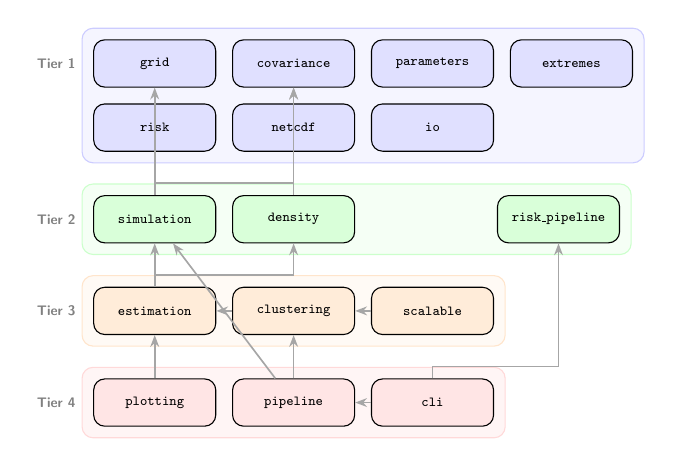
\begin{tikzpicture}[
  module/.style={draw, rounded corners, minimum width=1.55cm, minimum height=0.6cm,
    font=\ttfamily\tiny, align=center},
  tier1/.style={module, fill=blue!12},
  tier2/.style={module, fill=green!15},
  tier3/.style={module, fill=orange!15},
  tier4/.style={module, fill=red!10},
  arr/.style={-{Stealth[length=1.5mm]}, semithick, gray!70},
  tierlab/.style={font=\sffamily\tiny\bfseries, text=gray},
  node distance=0.25cm and 0.2cm,
]
% --- Tier 1: Core math, row 1 (4 modules) ---
\node[tier1] (grid)        {grid};
\node[tier1, right=of grid] (cov)    {covariance};
\node[tier1, right=of cov]  (param)  {parameters};
\node[tier1, right=of param](extr)   {extremes};
% --- Tier 1: Core math, row 2 (3 modules) ---
\node[tier1, below=0.2cm of grid]  (risk)  {risk};
\node[tier1, right=of risk]        (nc)    {netcdf};
\node[tier1, right=of nc]          (iom)   {io};

% --- Tier 2: Simulation & estimation ---
\node[tier2, below=0.55cm of risk]  (sim)  {simulation};
\node[tier2, right=of sim]          (dens) {density};
\node[tier2, right=1.8cm of dens]   (rpipe){risk\_pipeline};

% --- Tier 3: Clustering & smoothing ---
\node[tier3, below=0.55cm of sim]   (est)  {estimation};
\node[tier3, right=of est]          (clust){clustering};
\node[tier3, right=of clust]        (scal) {scalable};

% --- Tier 4: Orchestration ---
\node[tier4, below=0.55cm of est]   (plot) {plotting};
\node[tier4, right=of plot]         (pipe) {pipeline};
\node[tier4, right=of pipe]         (cli)  {cli};

% --- Dependencies (arrows) ---
\draw[arr] (sim)  -- (grid);
\draw[arr] (sim.north)  -- ++(0,0.15) -| (cov.south);
\draw[arr] (dens.north) -- ++(0,0.15) -| (cov.south);
\draw[arr] (est)  -- (sim);
\draw[arr] (est.north)  -- ++(0,0.15) -| (dens.south);
\draw[arr] (clust)-- (est);
\draw[arr] (scal) -- (clust);
\draw[arr] (pipe) -- (sim);
\draw[arr] (pipe.north) -- ++(0,0.15) -| (clust.south);
\draw[arr] (cli)  -- (pipe);
\draw[arr] (cli.north)  -- ++(0,0.15) -| (rpipe.south);
\draw[arr] (plot) -- (est);

% --- Tier labels ---
\node[tierlab, left=0.1cm of grid]   {Tier 1};
\node[tierlab, left=0.1cm of sim]    {Tier 2};
\node[tierlab, left=0.1cm of est]    {Tier 3};
\node[tierlab, left=0.1cm of plot]   {Tier 4};

% --- Background boxes ---
\begin{scope}[on background layer]
  \node[fit=(grid)(extr)(risk)(iom), fill=blue!4, draw=blue!20, rounded corners, inner sep=4pt] {};
  \node[fit=(sim)(rpipe), fill=green!4, draw=green!20, rounded corners, inner sep=4pt] {};
  \node[fit=(est)(scal), fill=orange!4, draw=orange!20, rounded corners, inner sep=4pt] {};
  \node[fit=(plot)(cli), fill=red!4, draw=red!15, rounded corners, inner sep=4pt] {};
\end{scope}
\end{tikzpicture}%
}% end resizebox
\caption{Module dependency structure of \texttt{weatherisk}.
  Tier~1 modules have no inter-package dependencies;
  higher tiers depend only on modules in the same or lower tiers.
  Arrows indicate \texttt{import} dependencies.}
\label{fig:architecture}
\end{figure}

\subsection{Software functionalities}
\label{sec:functionalities}

\subsubsection{Covariance model}

The stationary anisotropic covariance function is
\begin{equation}\label{eq:cov-stat}
  C(\mathbf{h}) = \exp\!\bigl(-\|\Sigma^{-1}\mathbf{h}\|^{\alpha}\bigr),
\end{equation}
where $\mathbf{h} = (x, y)^T$ is the spatial lag,
$\alpha \in (0, 2]$ is the smoothness exponent, and the precision matrix
\begin{equation}\label{eq:sigma-inv}
  \Sigma^{-1} = R(\gamma)
  \begin{pmatrix} 1/a & 0 \\ 0 & 1/(a+b) \end{pmatrix}
  R(\gamma)^T
\end{equation}
encodes ellipse semi-axes $a > 0$, $a + b$ (semi-major), and rotation
angle~$\gamma$.

The non-stationary variant blends two anisotropy matrices
$M_1, M_2$ (the inverse covariance matrices at locations~1 and~2)
through the harmonic mean:
\begin{equation}\label{eq:omega}
  \Omega = \Bigl(\frac{M_1^{-1} + M_2^{-1}}{2}\Bigr)^{-1},
\end{equation}
\begin{equation}\label{eq:cov-nonstat}
  C_{\mathrm{ns}}(\mathbf{h}) = \min\!\Bigl(1,\;
    \sqrt{\det(\Omega)\,a_1(a_1+b_1)\,a_2(a_2+b_2)}\;
    \exp\!\bigl(-\sqrt{\mathbf{h}^T\Omega\,\mathbf{h}}^{\,\alpha}\bigr)\Bigr).
\end{equation}
When both parameter sets are identical, $\Omega = M_1$ and the prefactor
reduces to unity, recovering the stationary case.

\subsubsection{Extremal coefficient}

The extremal coefficient $\theta \in [1, 2]$ of the extremal-$t$ model
links pairwise dependence to correlation~$\rho$ via
\begin{equation}\label{eq:ec}
  \theta(\rho) = 2\, T_{\nu+1}\!\left(
    \sqrt{\frac{(\nu+1)(1-\rho)}{1+\rho}}\right),
\end{equation}
where $T_{\nu+1}$ is the CDF of the Student-$t$ distribution with
$\nu + 1$ degrees of freedom.
At $\rho = 0$ with finite $\nu$, $\theta < 2$ (residual tail dependence);
complete independence ($\theta = 2$) is reached only as $\nu \to \infty$.

\subsubsection{Max-stable process simulation}

Simulation follows the spectral representation of~\cite{schlather2002}:
a Poisson point process on $(0, \infty)$ with intensity $\zeta^{-2}\,d\zeta$
generates arrival times; for each arrival, a Gaussian spectral function
is drawn from the multivariate normal with covariance matrix obtained via
Cholesky decomposition of the grid covariance.
The pointwise maximum over all spectral functions, scaled by the Poisson
arrival, yields the max-stable realisation.
Margins are Student-$t$ with $\nu$ degrees of freedom, normalised to
unit Fr\'{e}chet via the probability integral transform.

\subsubsection{Pairwise composite likelihood estimation}

Local parameters $(a, b, \gamma)$ at each grid cell are estimated by
maximising the pairwise composite log-likelihood~\cite{padoan2010}:
\begin{equation}\label{eq:pcl}
  \ell(\theta) = \sum_{i < j} \log f(z_i, z_j; \theta),
\end{equation}
where the sum runs over all pairs within a spatial neighbourhood and
$f$ is the bivariate density implied by the covariance model.
Optimisation uses Latin Hypercube initialisation followed by
L-BFGS-B~\cite{byrd1995}.

\subsubsection{Clustering}

Two clustering methods are implemented:
\begin{enumerate}
\item \textbf{Ellipse dissimilarity}: For each pair of grid cells, the
  Jaccard-like overlap between estimated anisotropy ellipses is computed
  and scaled to a dissimilarity in $[0, 100]$. Hierarchical agglomerative
  clustering (average linkage) is applied, and $k$ is determined by a
  threshold on merge heights.
\item \textbf{Saunders method}: Rank-based madogram estimation of pairwise
  extremal coefficients yields an alternative dissimilarity
  matrix~\cite{saunders2021,cooley2006}.
\end{enumerate}

\subsubsection{Risk metrics}

Given cluster assignments, \texttt{weatherisk} computes per-cluster
tail-risk metrics on the Fr\'{e}chet scale.
For cluster~$A_k$, the loss series is the spatial block maximum
$L_t = \max_{s \in A_k} Z_t(s)$, where $Z_t(s)$ are the Fr\'{e}chet-transformed
annual maxima.  Then:
\begin{align}
  \mathrm{VaR}_p &= \inf\{x : P(L \leq x) \geq p\}, \label{eq:var} \\
  \mathrm{ES}_p  &= E[L \mid L > \mathrm{VaR}_p]. \label{eq:es}
\end{align}
These are hazard-intensity metrics: they quantify how severe the joint
extreme events are within each cluster on a standardised scale, rather
than in physical units.
The implementation validates $\mathrm{ES}_p \geq \mathrm{VaR}_p$
by construction.

\subsubsection{GDP exposure weighting}
\label{sec:gdp}

To connect statistical tail-risk to economic impact, \texttt{weatherisk}
optionally incorporates gridded GDP data from Kummu et al.~\cite{kummu2018}.
The GDP~PPP grid (5~arc-min, constant~2011~international~USD) is aggregated
onto the coarser pipeline grid by summing fine-resolution cells within
each coarse cell boundary.
The cell-level risk is then defined as
\begin{equation}\label{eq:risk-gdp}
  \mathrm{Risk}(s) = \mathrm{ES}_{95}^{k(s)} \times \mathrm{GDP}(s),
\end{equation}
where $k(s)$ is the cluster to which cell~$s$ belongs.
This avoids cluster-size bias: a city cell with high GDP within the
same cluster as a desert cell appropriately receives a higher risk
value despite sharing the same hazard intensity.

\subsubsection{Scalable clustering for global grids}

For grids exceeding $\sim$16\,000 cells, the full dissimilarity matrix
is prohibitively large.
\texttt{weatherisk} provides a coarse-grid proxy strategy, illustrated
in Figure~\ref{fig:scalable}.

\begin{figure}[ht]
\centering
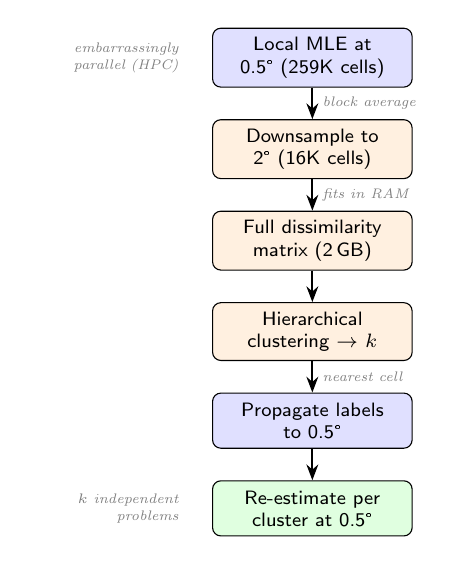
\begin{tikzpicture}[
  box/.style={draw, rounded corners=3pt, minimum width=2.4cm, minimum height=0.7cm,
    font=\sffamily\scriptsize, align=center, text width=2.3cm},
  fine/.style={box, fill=blue!12},
  coarse/.style={box, fill=orange!12},
  result/.style={box, fill=green!12},
  arr/.style={-{Stealth[length=2mm]}, thick},
  note/.style={font=\itshape\tiny, text=gray},
  node distance=0.4cm,
]

\node[fine]   (est)   {Local MLE at\\0.5\textdegree\ (259K cells)};
\node[coarse, below=of est] (down) {Downsample to\\2\textdegree\ (16K cells)};
\node[coarse, below=of down] (dmat) {Full dissimilarity\\matrix (2\,GB)};
\node[coarse, below=of dmat] (hclust) {Hierarchical\\clustering $\to$ $k$};
\node[fine,   below=of hclust] (prop) {Propagate labels\\to 0.5\textdegree};
\node[result, below=of prop] (reest) {Re-estimate per\\cluster at 0.5\textdegree};

\draw[arr] (est) -- (down) node[midway, right, note] {block average};
\draw[arr] (down) -- (dmat) node[midway, right, note] {fits in RAM};
\draw[arr] (dmat) -- (hclust);
\draw[arr] (hclust) -- (prop) node[midway, right, note] {nearest cell};
\draw[arr] (prop) -- (reest);

% HPC annotation
\node[note, left=0.3cm of est, text width=1.8cm, align=right]
  {embarrassingly\\parallel (HPC)};
\node[note, left=0.3cm of reest, text width=1.8cm, align=right]
  {$k$ independent\\problems};

\end{tikzpicture}
\caption{Coarse-grid proxy strategy for scalable clustering.
  Local estimation is embarrassingly parallel at full resolution;
  clustering operates on a downsampled grid that fits in memory;
  labels are propagated back and refined.}
\label{fig:scalable}
\end{figure}

Intermediate results are checkpointed via \texttt{save\_chunk}/\texttt{load\_chunk},
enabling SLURM job-array parallelism on HPC systems.

\subsection{Pipeline flows}

The CLI exposes four pipeline flows, illustrated in Figure~\ref{fig:flows}.

\begin{figure*}[ht]
\centering
\resizebox{\textwidth}{!}{%
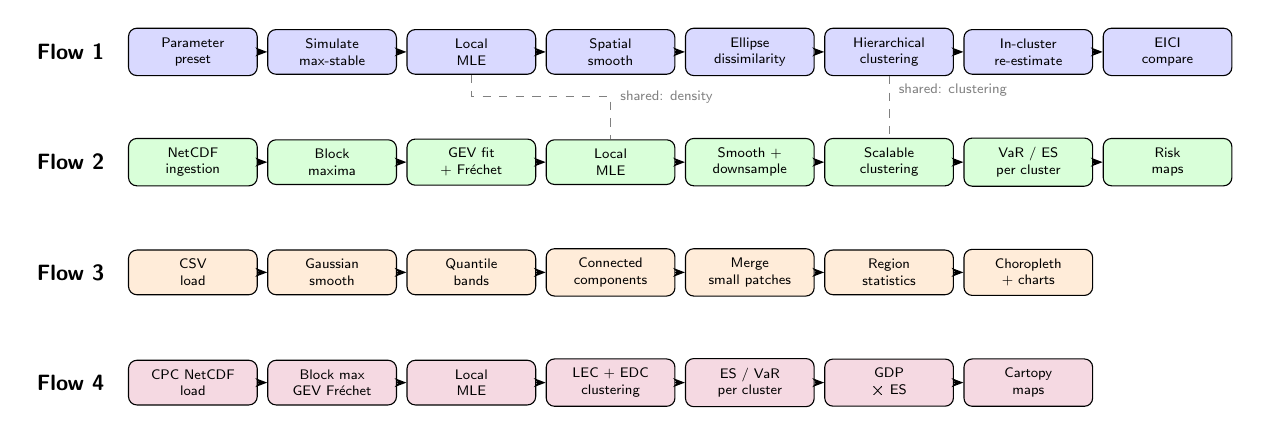
\begin{tikzpicture}[
  stepbox/.style={draw, rounded corners=3pt, minimum width=1.5cm, minimum height=0.55cm,
    font=\sffamily\tiny, align=center, text width=1.4cm},
  flow1/.style={stepbox, fill=blue!15},
  flow2/.style={stepbox, fill=green!15},
  flow3/.style={stepbox, fill=orange!15},
  arr/.style={-{Stealth[length=1.5mm]}, semithick},
  flowlabel/.style={font=\sffamily\footnotesize\bfseries, anchor=east},
  node distance=0.12cm and 0.12cm,
]

% ===== FLOW 1: Validation =====
\node[flowlabel] at (-0.5, 0) {Flow 1};
\node[flow1] (f1a) at (0.5,0) {Parameter\\preset};
\node[flow1, right=of f1a] (f1b) {Simulate\\max-stable};
\node[flow1, right=of f1b] (f1c) {Local\\MLE};
\node[flow1, right=of f1c] (f1d) {Spatial\\smooth};
\node[flow1, right=of f1d] (f1e) {Ellipse\\dissimilarity};
\node[flow1, right=of f1e] (f1f) {Hierarchical\\clustering};
\node[flow1, right=of f1f] (f1g) {In-cluster\\re-estimate};
\node[flow1, right=of f1g] (f1h) {EICI\\compare};

\draw[arr] (f1a) -- (f1b);
\draw[arr] (f1b) -- (f1c);
\draw[arr] (f1c) -- (f1d);
\draw[arr] (f1d) -- (f1e);
\draw[arr] (f1e) -- (f1f);
\draw[arr] (f1f) -- (f1g);
\draw[arr] (f1g) -- (f1h);

% ===== FLOW 2: Real-data risk =====
\node[flowlabel] at (-0.5, -1.4) {Flow 2};
\node[flow2] (f2a) at (0.5,-1.4) {NetCDF\\ingestion};
\node[flow2, right=of f2a] (f2b) {Block\\maxima};
\node[flow2, right=of f2b] (f2c) {GEV fit\\+ Fr\'{e}chet};
\node[flow2, right=of f2c] (f2d) {Local\\MLE};
\node[flow2, right=of f2d] (f2e) {Smooth +\\downsample};
\node[flow2, right=of f2e] (f2f) {Scalable\\clustering};
\node[flow2, right=of f2f] (f2g) {VaR / ES\\per cluster};
\node[flow2, right=of f2g] (f2h) {Risk\\maps};

\draw[arr] (f2a) -- (f2b);
\draw[arr] (f2b) -- (f2c);
\draw[arr] (f2c) -- (f2d);
\draw[arr] (f2d) -- (f2e);
\draw[arr] (f2e) -- (f2f);
\draw[arr] (f2f) -- (f2g);
\draw[arr] (f2g) -- (f2h);

% ===== FLOW 3: Risk pipeline =====
\node[flowlabel] at (-0.5, -2.8) {Flow 3};
\node[flow3] (f3a) at (0.5,-2.8) {CSV\\load};
\node[flow3, right=of f3a] (f3b) {Gaussian\\smooth};
\node[flow3, right=of f3b] (f3c) {Quantile\\bands};
\node[flow3, right=of f3c] (f3d) {Connected\\components};
\node[flow3, right=of f3d] (f3e) {Merge\\small patches};
\node[flow3, right=of f3e] (f3f) {Region\\statistics};
\node[flow3, right=of f3f] (f3g) {Choropleth\\+ charts};

\draw[arr] (f3a) -- (f3b);
\draw[arr] (f3b) -- (f3c);
\draw[arr] (f3c) -- (f3d);
\draw[arr] (f3d) -- (f3e);
\draw[arr] (f3e) -- (f3f);
\draw[arr] (f3f) -- (f3g);

% ===== FLOW 4: CPC Maps =====
\node[flowlabel] at (-0.5, -4.2) {Flow 4};
\node[flow2, fill=purple!15] (f4a) at (0.5,-4.2) {CPC NetCDF\\load};
\node[flow2, fill=purple!15, right=of f4a] (f4b) {Block max\\GEV Fr\'{e}chet};
\node[flow2, fill=purple!15, right=of f4b] (f4c) {Local\\MLE};
\node[flow2, fill=purple!15, right=of f4c] (f4d) {LEC + EDC\\clustering};
\node[flow2, fill=purple!15, right=of f4d] (f4e) {ES / VaR\\per cluster};
\node[flow2, fill=purple!15, right=of f4e] (f4f) {GDP\\\texttimes\ ES};
\node[flow2, fill=purple!15, right=of f4f] (f4g) {Cartopy\\maps};

\draw[arr] (f4a) -- (f4b);
\draw[arr] (f4b) -- (f4c);
\draw[arr] (f4c) -- (f4d);
\draw[arr] (f4d) -- (f4e);
\draw[arr] (f4e) -- (f4f);
\draw[arr] (f4f) -- (f4g);

% ===== Shared modules annotation =====
\draw[dashed, gray] (f1c.south) -- ++(0,-0.28) -| (f2d.north)
  node[midway, right, font=\sffamily\tiny, text=gray] {shared: density};
\draw[dashed, gray] (f1f.south) -- ++(0,-0.18) -| (f2f.north)
  node[midway, right, font=\sffamily\tiny, text=gray] {shared: clustering};

\end{tikzpicture}%
}% end resizebox
\caption{The four pipeline flows of \texttt{weatherisk}.
  Flow~1 validates the method on synthetic data.
  Flow~2 applies the full method to real climate observations with risk metrics.
  Flow~3 provides lightweight post-processing of pre-computed risk maps.
  Flow~4 runs the complete LEC/EDC pipeline on NOAA CPC data with optional
  GDP exposure weighting and generates filled-region Cartopy maps.
  Dashed lines indicate shared modules between flows.}
\label{fig:flows}
\end{figure*}

\paragraph{Flow~1: Method validation (\texttt{weatherisk validate}).}
Reproduces the clustering method on synthetic data:
parameters $\to$ simulate $\to$ local estimation $\to$ smooth $\to$
ellipse dissimilarity $\to$ hierarchical clustering $\to$ in-cluster
re-estimation.
Grid sizes of 10--51 points per axis run in minutes on a laptop.

\begin{lstlisting}[caption={Running the validation flow.},label=lst:validate]
$ weatherisk validate --params stripes \
    --resolution 10 --n-sim 20 \
    --seed 42
\end{lstlisting}

\paragraph{Flow~2: Real-data risk analysis (\texttt{weatherisk risk}).}
Applies the method to observed climate data (CPC, ERA5):
NetCDF ingestion $\to$ block maxima $\to$ GEV fit $\to$ Fr\'{e}chet
transform $\to$ local MLE $\to$ smooth $\to$ scalable clustering
$\to$ VaR/ES per cluster $\to$ plots.

\begin{lstlisting}[caption={Running the risk analysis flow.},label=lst:risk]
$ weatherisk risk \
    --netcdf \
    data/cpc_tmax.nc \
    --hazard heat \
    -k 25 --workers 8
\end{lstlisting}

\paragraph{Flow~3: Risk pipeline.}
\begin{sloppypar}
\texttt{weatherisk risk\-pipe\-line}---lightweight
post-processing of pre-computed risk maps:
CSV $\to$ Gaussian smoothing $\to$ quantile banding $\to$
connected-component labelling $\to$ merge small patches
$\to$ per-region statistics.
\end{sloppypar}

\begin{lstlisting}[caption={Running the risk pipeline.},label=lst:riskpipe]
$ weatherisk risk-pipeline \
    --csv data/risk_map_grid.csv \
    --bands 6
\end{lstlisting}

\paragraph{Flow~4: CPC maps (\texttt{weatherisk maps}).}
The primary pipeline for reproducible analysis of NOAA CPC daily climate
data.  Loads 20~years of NetCDF files, computes annual block maxima,
fits GEV marginals, transforms to unit Fr\'{e}chet, performs local MLE of
anisotropy parameters $(a, b, \gamma)$, runs both LEC and EDC clustering,
and outputs filled-region Cartopy maps.
When a GDP path is provided, computes cell-level exposure-weighted risk
(Equation~\ref{eq:risk-gdp}).

\begin{lstlisting}[caption={Running the CPC maps pipeline with GDP exposure.},label=lst:maps]
$ weatherisk maps \
    --variable precip \
    --gdp-path data/gdp/GDP_PPP.nc
\end{lstlisting}

%% ============================================================
\section{Illustrative examples}
\label{sec:examples}
%% ============================================================

Figure~\ref{fig:math-workflow} illustrates the mathematical transformation
chain from raw observations to risk metrics.

\begin{figure}[ht]
\centering
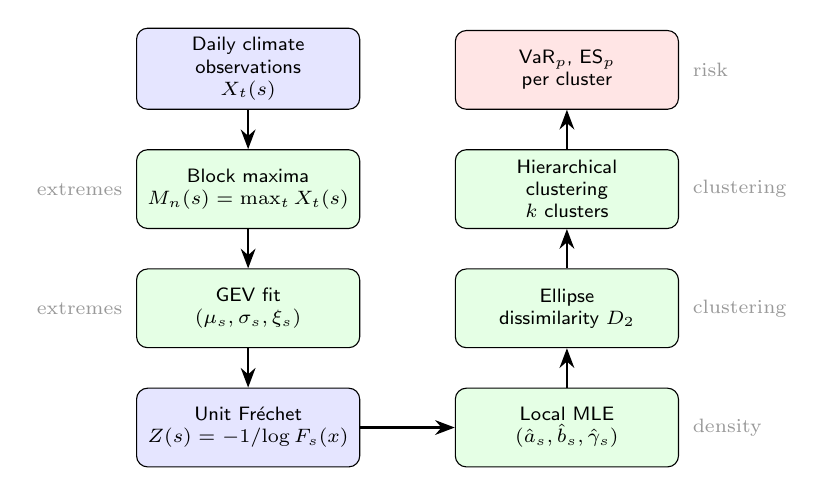
\begin{tikzpicture}[
  box/.style={draw, rounded corners=4pt, minimum width=2.8cm, minimum height=1.0cm,
    font=\sffamily\scriptsize, align=center, text width=2.6cm},
  data/.style={box, fill=blue!10},
  proc/.style={box, fill=green!10},
  outbox/.style={box, fill=red!10},
  arr/.style={-{Stealth[length=2.5mm]}, thick},
  eq/.style={font=\scriptsize, text=gray!80},
  node distance=0.5cm,
]

% Left column: Data transformations
\node[data] (raw) {Daily climate\\observations\\$X_t(s)$};
\node[proc, below=of raw] (bm) {Block maxima\\$M_n(s) = \max_{t} X_t(s)$};
\node[proc, below=of bm] (gev) {GEV fit\\$(\mu_s, \sigma_s, \xi_s)$};
\node[data, below=of gev] (frech) {Unit Fr\'{e}chet\\$Z(s) = -1/\!\log F_s(x)$};

% Right column: Estimation → Clustering → Risk
\node[proc, right=1.2cm of frech] (mle) {Local MLE\\$(\hat{a}_s, \hat{b}_s, \hat{\gamma}_s)$};
\node[proc, above=of mle] (diss) {Ellipse\\dissimilarity $D_2$};
\node[proc, above=of diss] (clust) {Hierarchical\\clustering\\$k$ clusters};
\node[outbox, above=of clust]  (risk) {VaR$_p$, ES$_p$\\per cluster};

% Arrows
\draw[arr] (raw) -- (bm);
\draw[arr] (bm) -- (gev);
\draw[arr] (gev) -- (frech);
\draw[arr] (frech) -- (mle);
\draw[arr] (mle) -- (diss);
\draw[arr] (diss) -- (clust);
\draw[arr] (clust) -- (risk);

% Equation annotations
\node[eq, left=0.05cm of bm, anchor=east] {extremes};
\node[eq, left=0.05cm of gev, anchor=east] {extremes};
\node[eq, right=0.05cm of mle, anchor=west] {density};
\node[eq, right=0.05cm of diss, anchor=west] {clustering};
\node[eq, right=0.05cm of clust, anchor=west] {clustering};
\node[eq, right=0.05cm of risk, anchor=west] {risk};

\end{tikzpicture}
\caption{Mathematical transformation chain in Flow~2.
  Left column: marginal transformations from raw observations to
  unit Fr\'{e}chet margins.
  Right column: dependence estimation, clustering, and risk quantification.
  Labels indicate the \texttt{weatherisk} module responsible for each step.}
\label{fig:math-workflow}
\end{figure}

\subsection{Synthetic validation}

We demonstrate Flow~1 on the ``stripes'' parameter preset, where the
semi-major axis~$b$ varies linearly with the $x$-coordinate, creating
stripe-like anisotropy regions that the clustering method should recover.

\begin{lstlisting}[caption={Python API usage for synthetic validation.},label=lst:api]
from weatherisk.parameters import get_preset
from weatherisk.pipeline import run_pipeline
from weatherisk.plotting import plot_cluster_map

p = get_preset("stripes")
result = run_pipeline(
    resolution=10, n_sim=20,
    df=p.df, alpha=p.alpha, seed=42,
)
fig = plot_cluster_map(
    result["clusters"], result["grid"]
)
fig.savefig("clusters.pdf")
\end{lstlisting}

The pipeline produces cluster assignments that align with the known
ground-truth anisotropy boundaries.
On a standard laptop (Apple M2, 16\,GB RAM), the 10$\times$10 grid
with 20~simulations completes in under 10~seconds.

Figure~\ref{fig:clustering-comparison} illustrates the two clustering
approaches.
Placeholder panels will be replaced by generated output plots
(see Section~\ref{sec:generated-plots}).

\begin{figure}[ht]
\centering
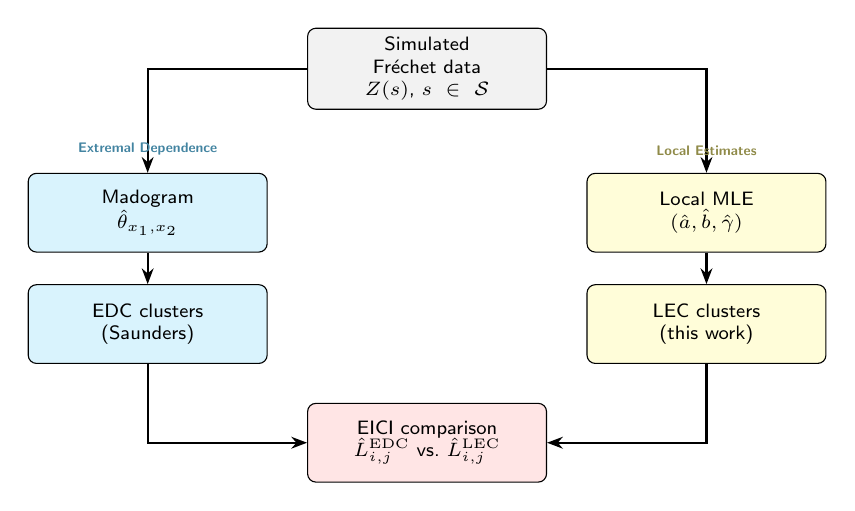
\begin{tikzpicture}[
  box/.style={draw, rounded corners=3pt, minimum width=3.0cm, minimum height=1.0cm,
    font=\sffamily\scriptsize, align=center, text width=2.8cm},
  input/.style={box, fill=gray!10},
  edc/.style={box, fill=cyan!15},
  lec/.style={box, fill=yellow!15},
  compare/.style={box, fill=red!10},
  arr/.style={-{Stealth[length=2mm]}, thick},
  node distance=0.4cm and 0.8cm,
]

% Input
\node[input] (sim) {Simulated\\Fr\'{e}chet data\\$Z(s)$, $s \in \mathcal{S}$};

% EDC branch (left)
\node[edc, below left=0.8cm and 0.5cm of sim] (mad) {Madogram\\$\hat{\theta}_{x_1,x_2}$};
\node[edc, below=of mad] (edc_clust) {EDC clusters\\(Saunders)};

% LEC branch (right)
\node[lec, below right=0.8cm and 0.5cm of sim] (mle) {Local MLE\\$(\hat{a}, \hat{b}, \hat{\gamma})$};
\node[lec, below=of mle] (lec_clust) {LEC clusters\\(this work)};

% Comparison
\node[compare, below=1.0cm of $(edc_clust)!0.5!(lec_clust)$] (eici)
  {EICI comparison\\$\hat{L}^{\mathrm{EDC}}_{i,j}$ vs.\ $\hat{L}^{\mathrm{LEC}}_{i,j}$};

% Arrows
\draw[arr] (sim) -| (mad);
\draw[arr] (sim) -| (mle);
\draw[arr] (mad) -- (edc_clust);
\draw[arr] (mle) -- (lec_clust);
\draw[arr] (edc_clust) |- (eici);
\draw[arr] (lec_clust) |- (eici);

% Labels
\node[font=\sffamily\tiny\bfseries, text=cyan!60!black, above=0.1cm of mad]
  {Extremal Dependence};
\node[font=\sffamily\tiny\bfseries, text=yellow!50!black, above=0.1cm of mle]
  {Local Estimates};

\end{tikzpicture}
\caption{Comparison of the two clustering approaches.
  EDC (left) uses madogram-based extremal coefficients;
  LEC (right, this work) uses locally estimated ellipse parameters.
  The EICI metric compares goodness of fit on cluster intersections,
  following~\cite{justus2024}.}
\label{fig:clustering-comparison}
\end{figure}

\subsection{Risk-map post-processing}

Flow~3 processes the included sample risk map
(\texttt{data/risk\_map\_grid.csv}), which contains latitude, longitude,
VaR$_{95}$, and ES$_{95}$ values on a global 0.5$^\circ$ grid.

\begin{lstlisting}[caption={Risk pipeline post-processing.},label=lst:postproc]
from weatherisk.risk_pipeline import (
    load_and_grid, smooth_field,
    quantile_bands, connected_patches,
    merge_tiny_regions,
    remap_ids_to_sequential,
    compute_cluster_stats,
)

data = load_and_grid("data/risk_map_grid.csv")
ES_s = smooth_field(
    data["ES"], sigma=0.8,
    land_mask=data["land_mask"],
)
bands, _ = quantile_bands(ES_s, n_bands=6)
clust = connected_patches(bands, min_patch=30)
clust = merge_tiny_regions(
    clust, data["lon_grid"], data["lat_grid"]
)
clust, K = remap_ids_to_sequential(clust)
print(f"Identified {K} risk regions")
\end{lstlisting}

%% NOTE: The following synthetic-data figures are generated by running
%% weatherisk validate --preset stripes/rotate/bigsmall.
%% They are commented out here because the simulation presets have not
%% yet been executed in this workspace.  Uncomment after running the
%% validate command to produce the PNG files in docs/figures/.

%% \subsection{Generated output plots}
%% \label{sec:generated-plots}
%%
%% The following figures are produced by running \texttt{weatherisk} on synthetic
%% data using the three parameter presets from~\cite{justus2024}.
%% Each row shows the EDC result (a), LEC result (b), and true parameter
%% field (c), reproducing and extending the figures from the original paper.
%%
%% \begin{figure}[ht]
%% \centering
%% 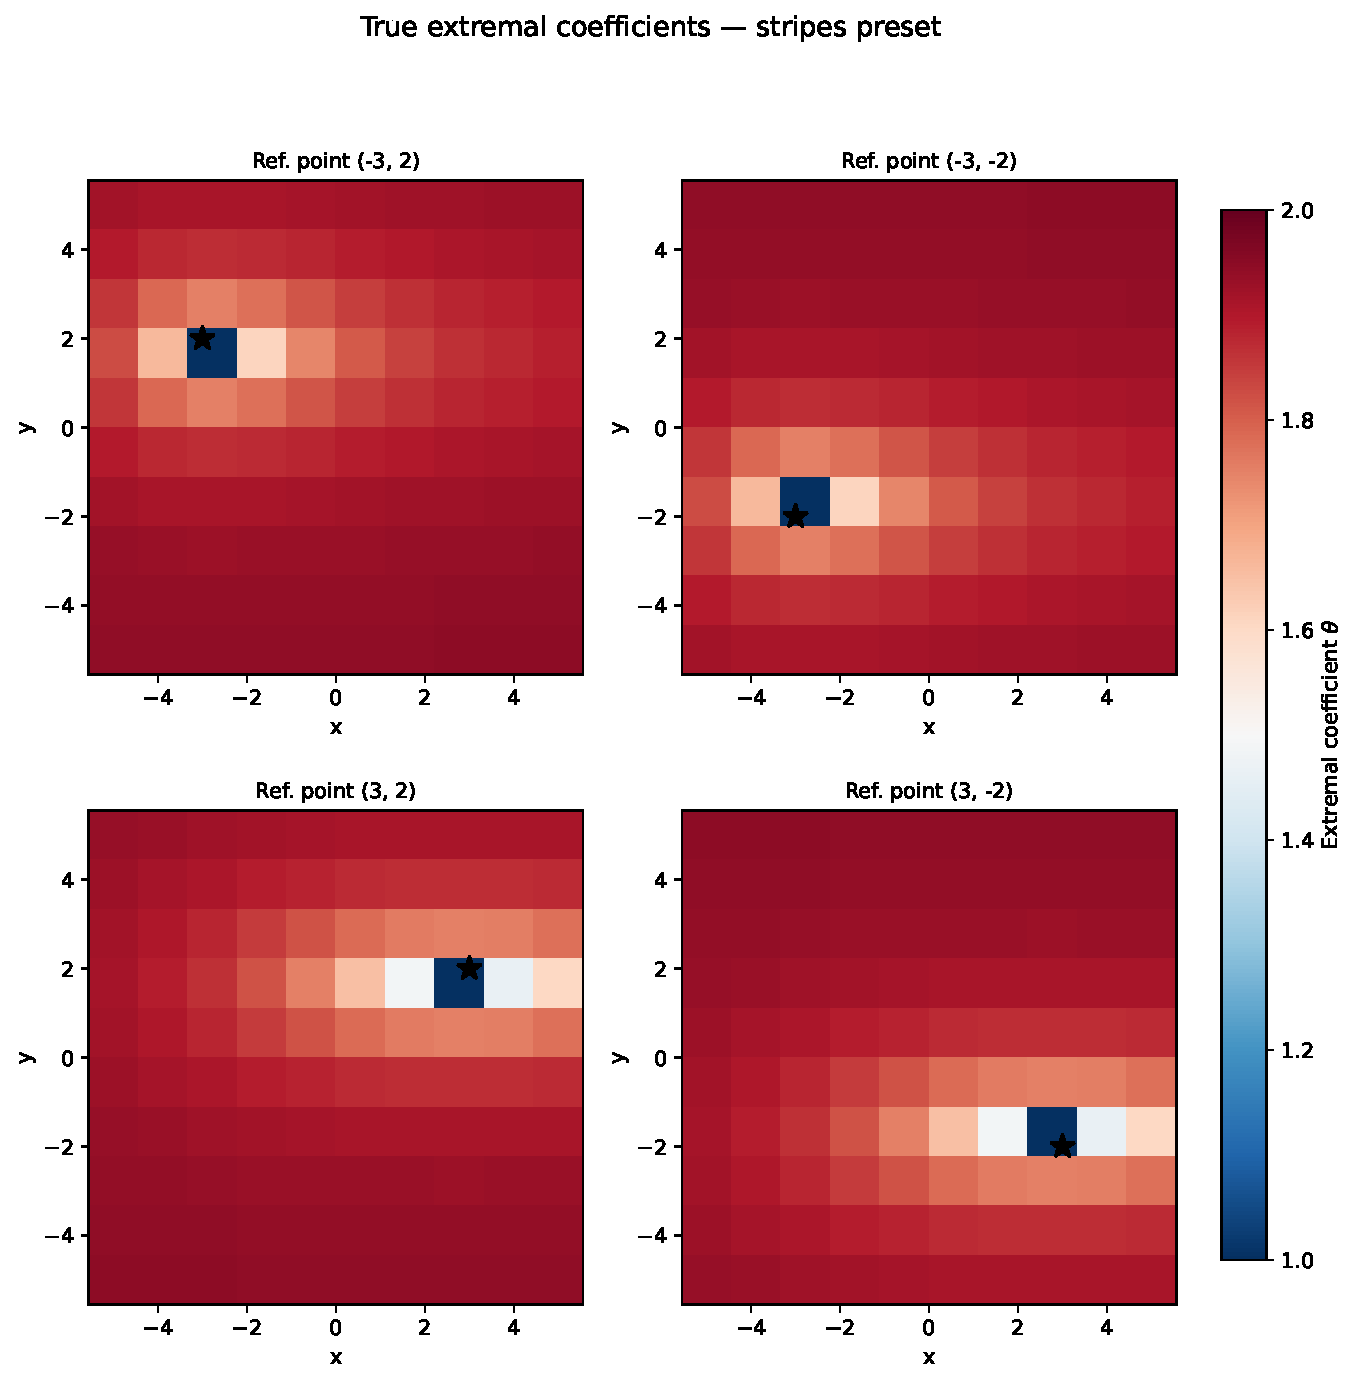
\includegraphics[width=0.95\textwidth]{figures/stripes_ec_maps.png}
%% \caption{True extremal coefficients $\theta$ for four reference points.}
%% \label{fig:ec-maps}
%% \end{figure}
%%
%% \begin{figure*}[ht]
%% \centering
%% 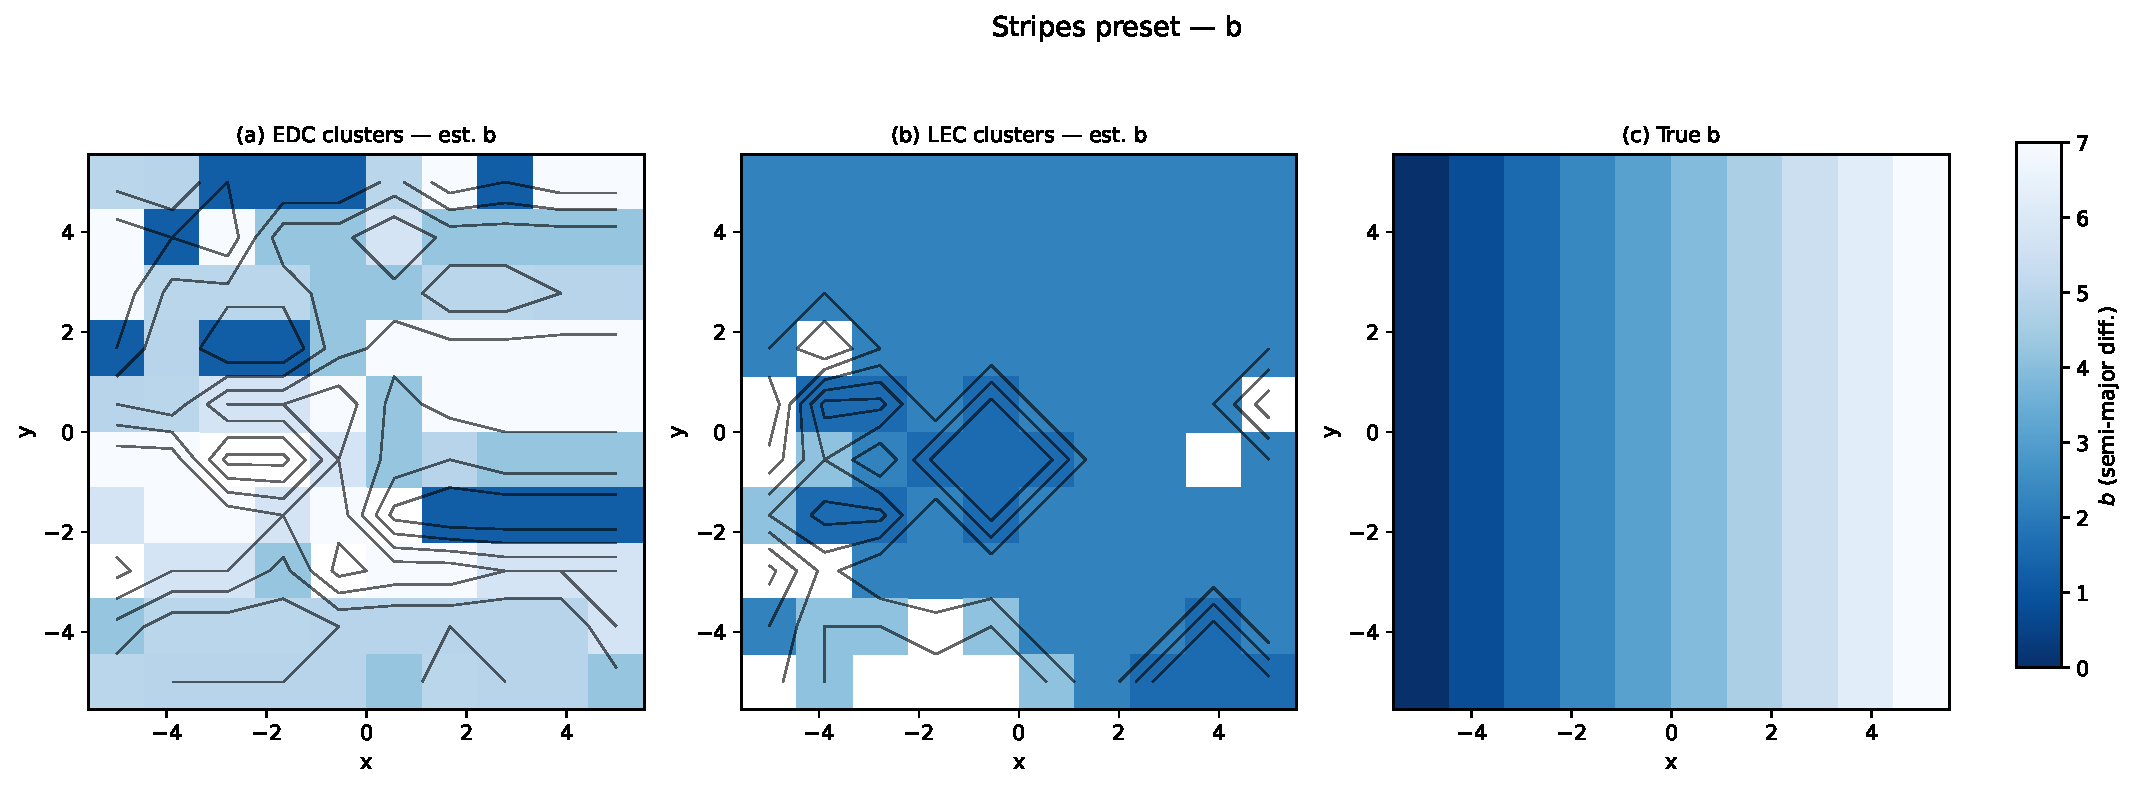
\includegraphics[width=0.95\textwidth]{figures/stripes_clusters_b.png}
%% \caption{Stripes preset: EDC/LEC clusters coloured by estimated~$b$.}
%% \label{fig:stripes-clusters}
%% \end{figure*}
%%
%% \begin{figure*}[ht]
%% \centering
%% 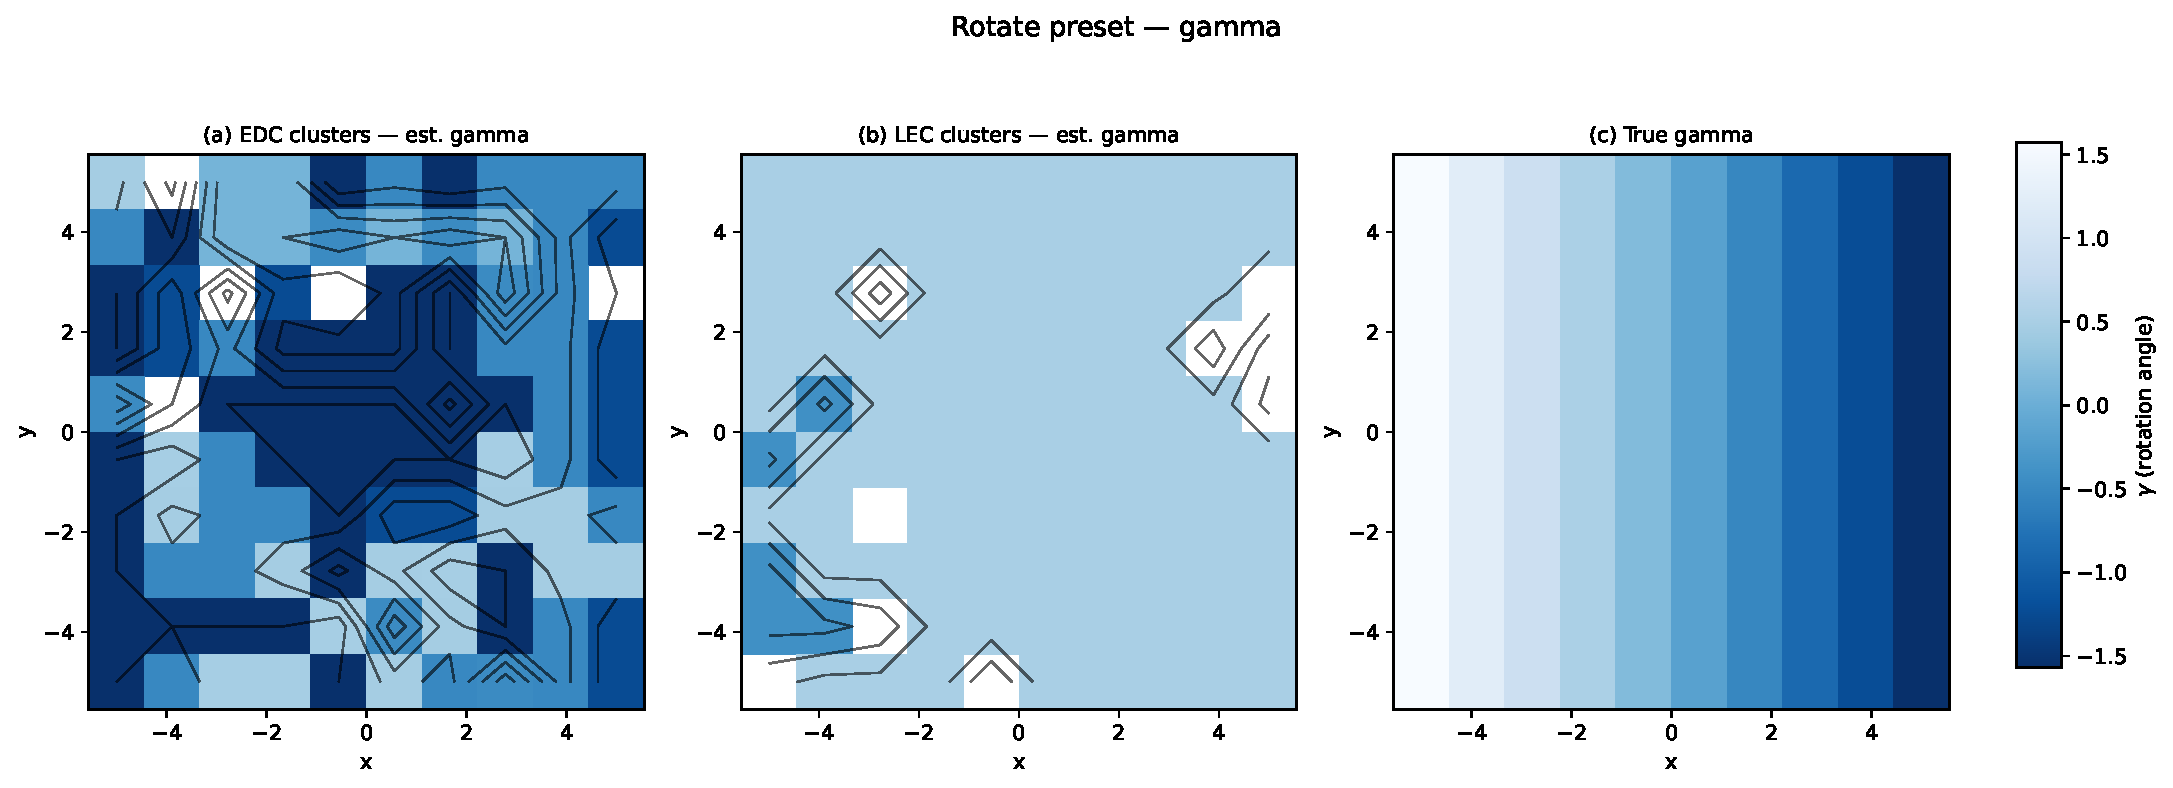
\includegraphics[width=0.95\textwidth]{figures/rotate_clusters_gamma.png}
%% \caption{Rotate preset: EDC/LEC clusters coloured by estimated~$\gamma$.}
%% \label{fig:rotate-clusters}
%% \end{figure*}
%%
%% \begin{figure*}[ht]
%% \centering
%% 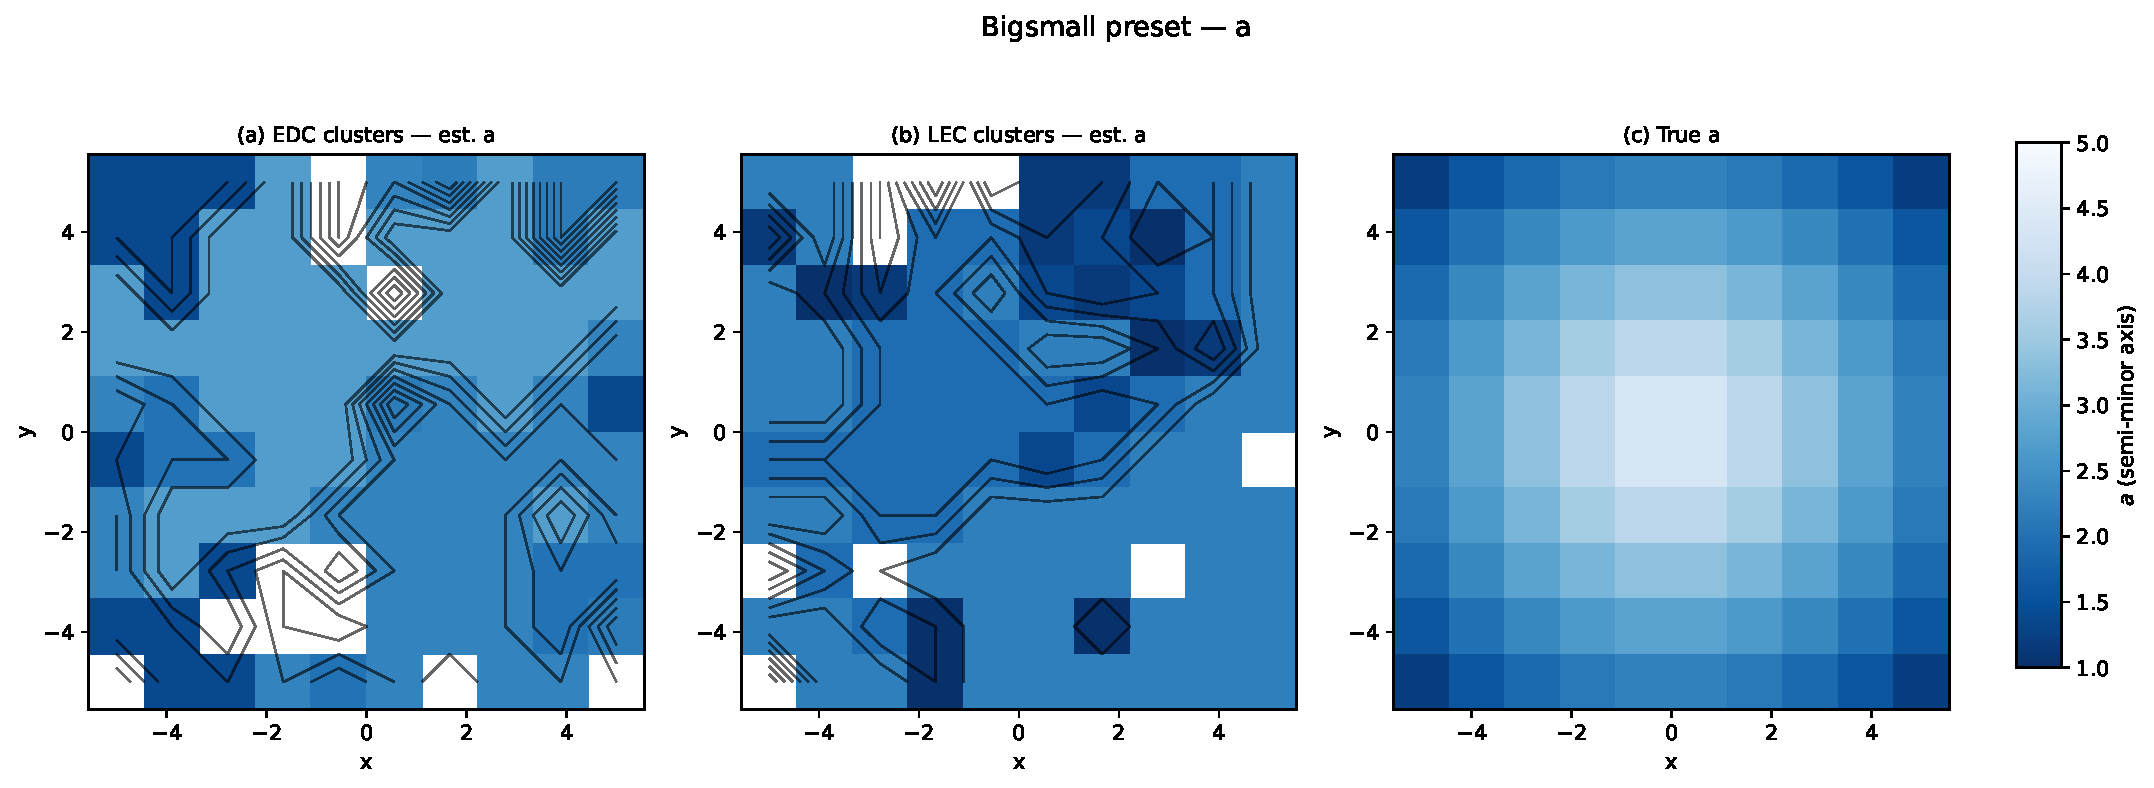
\includegraphics[width=0.95\textwidth]{figures/bigsmall_clusters_a.png}
%% \caption{Bigsmall preset: EDC/LEC clusters coloured by estimated~$a$.}
%% \label{fig:bigsmall-clusters}
%% \end{figure*}
%%
%% \begin{figure}[ht]
%% \centering
%% 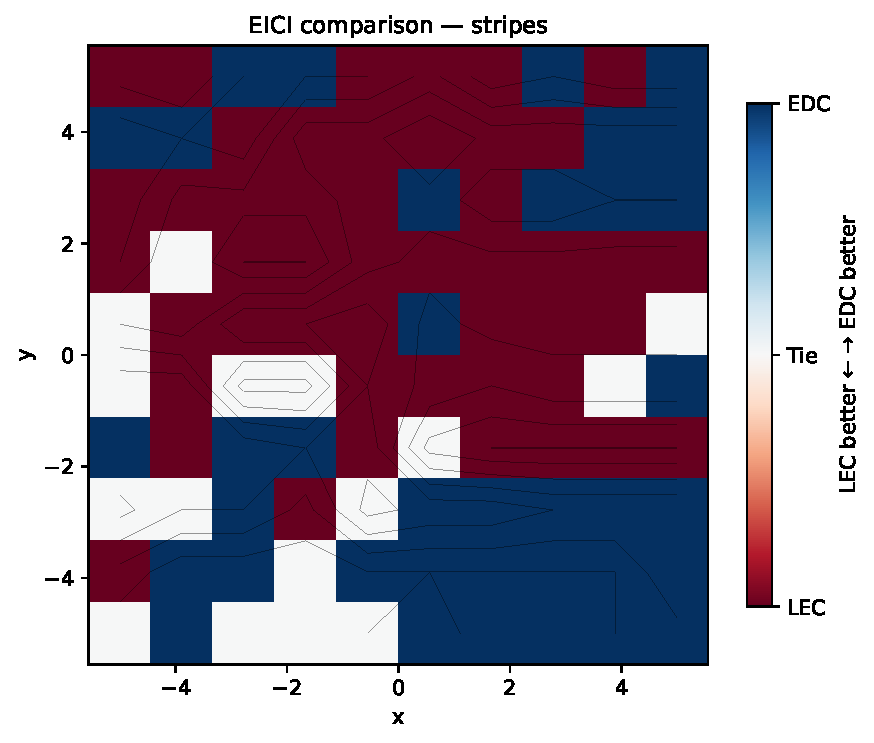
\includegraphics[width=0.65\textwidth]{figures/stripes_eici.png}
%% \caption{EICI goodness-of-fit comparison for the stripes preset.}
%% \label{fig:eici}
%% \end{figure}
%%
%% \begin{figure}[ht]
%% \centering
%% 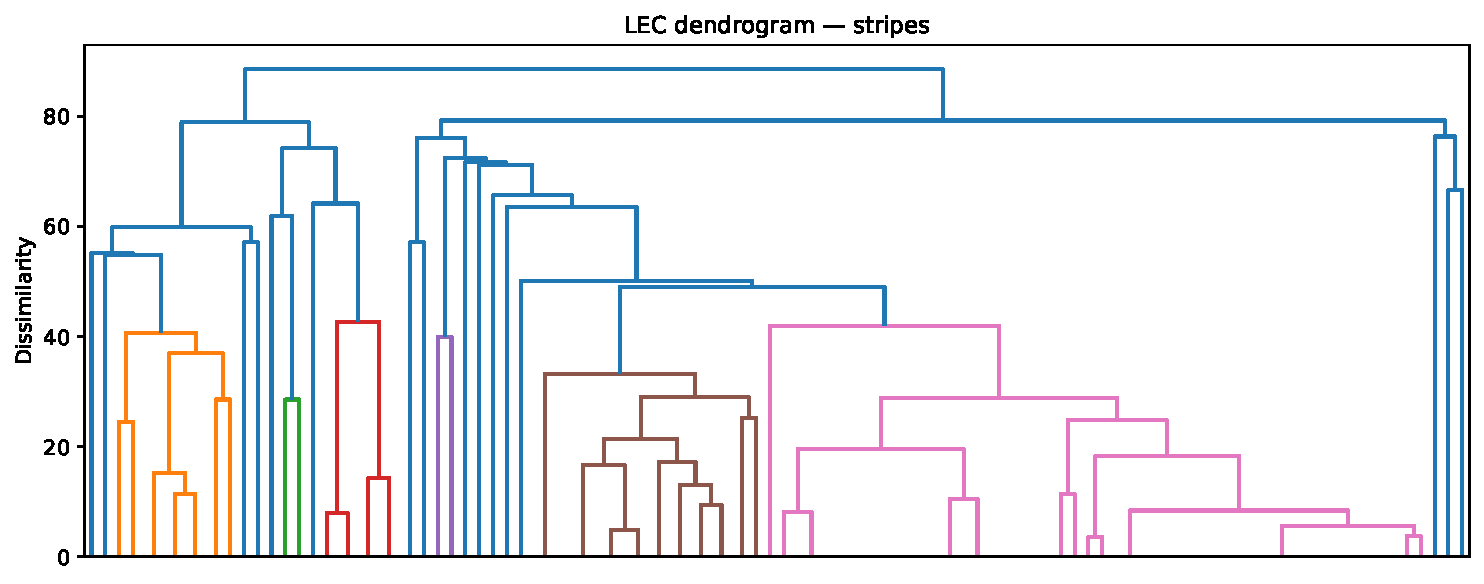
\includegraphics[width=0.85\textwidth]{figures/stripes_dendrogram.png}
%% \caption{LEC dendrogram for the stripes preset.}
%% \label{fig:dendrogram}
%% \end{figure}

\subsection{Real-data application: CPC precipitation}
\label{sec:real-data}

Flow~4 is applied to 20~years (2000--2019) of NOAA CPC daily
precipitation data over a European--Middle Eastern sub-region
(30\textdegree--65\textdegree N, 5\textdegree--55\textdegree E),
coarsened to $\sim$2\textdegree\ resolution (384~valid land cells).
Annual block maxima are computed, GEV marginals fitted, and values
transformed to unit Fr\'{e}chet margins.  Local pairwise composite
likelihood estimation yields anisotropy parameters $(a, b, \gamma)$
at each cell, which are spatially smoothed and used for both LEC
(ellipse-overlap $D_2$) and EDC (madogram $D_1$) clustering with
a 30\%-quantile threshold on the pairwise dissimilarity matrix.

The LEC method identifies $k = 26$ clusters and the EDC method
identifies $k = 18$ clusters.  Per-cluster tail-risk is quantified
by the Expected Shortfall at the 95th percentile (ES$_{95}$) of
the Fr\'{e}chet-scale spatial block maximum within each cluster.
This is a hazard-intensity metric that captures how severe the
joint extreme precipitation events are within each dependence
region, on a standardised extreme-value scale.

Figure~\ref{fig:cpc-summary} shows the summary panel with cluster
maps, estimated parameters, and tail-risk intensity.
Figure~\ref{fig:cpc-lec-clusters} shows the LEC clusters in detail.

\begin{figure*}[ht]
\centering
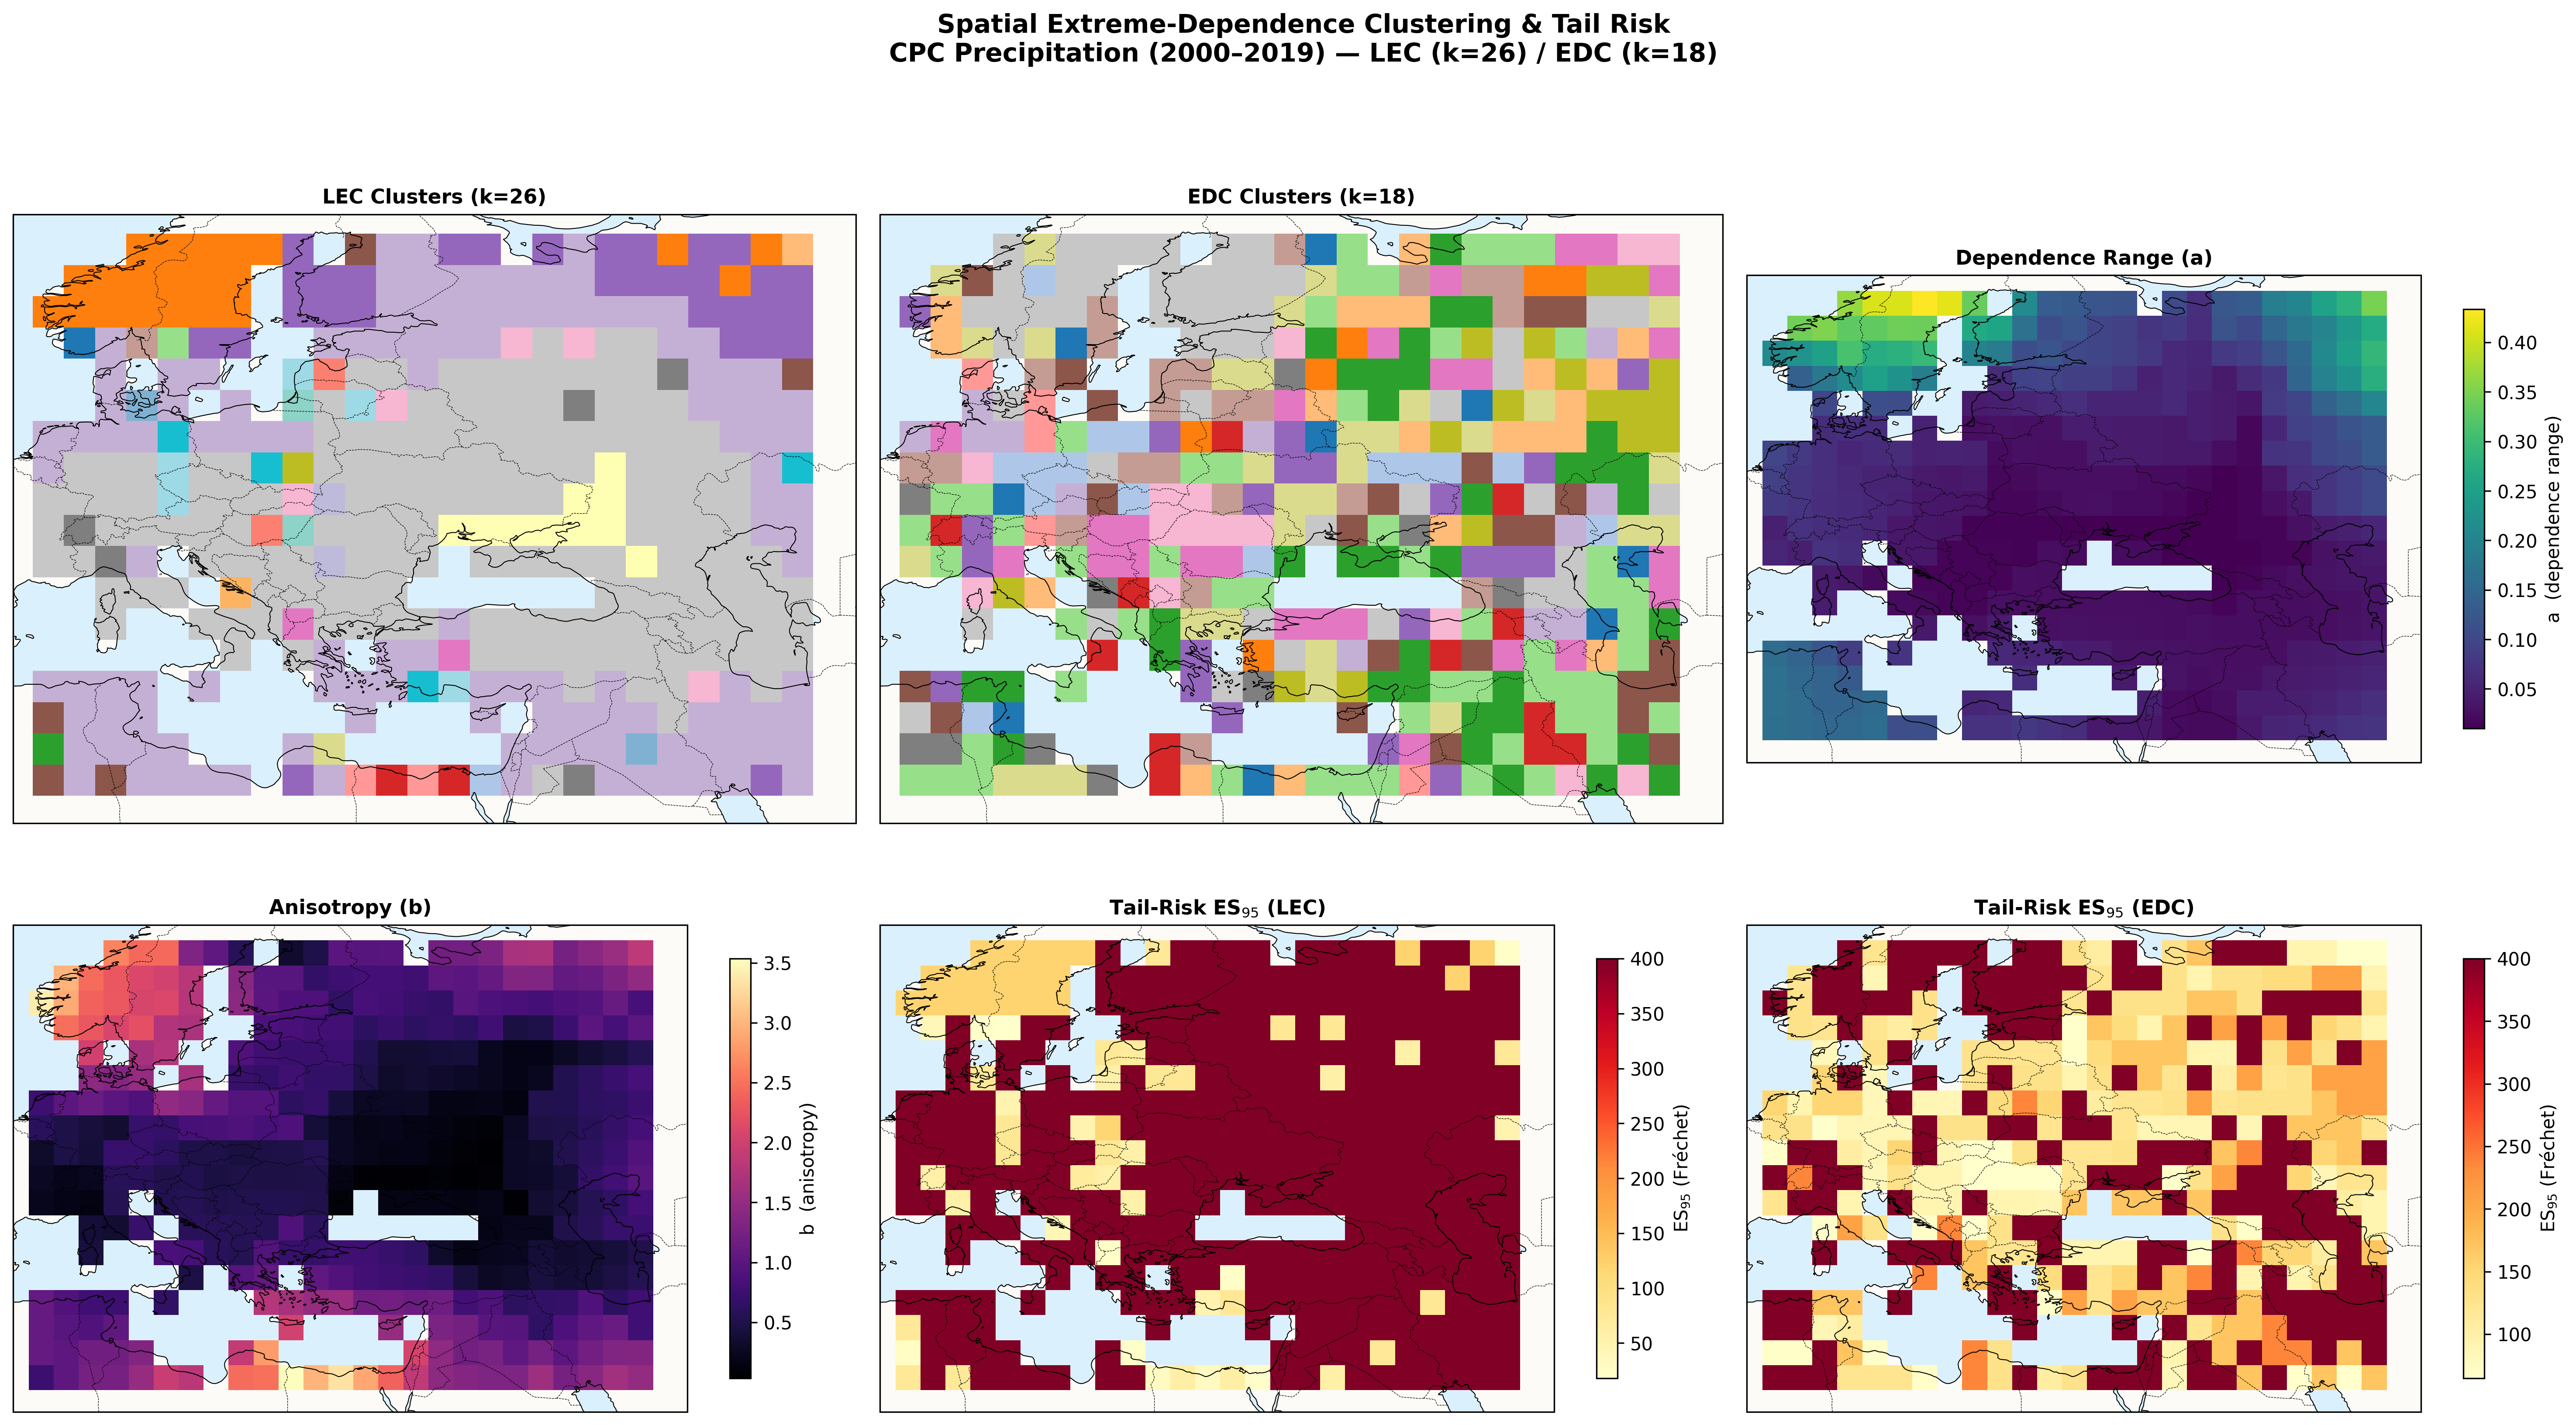
\includegraphics[width=0.95\textwidth]{figures/lec_edc_summary_panel.png}
\caption{Summary panel for CPC precipitation extremes (2000--2019).
  Top row: LEC clusters ($k = 26$), EDC clusters ($k = 18$),
  and estimated dependence range parameter~$a$.
  Bottom row: estimated anisotropy parameter~$b$,
  tail-risk intensity ES$_{95}$ for LEC clusters,
  and tail-risk intensity ES$_{95}$ for EDC clusters.
  The ES$_{95}$ values are on the Fr\'{e}chet scale: they measure
  the average severity of extreme events above the 95th percentile
  of the spatial block maximum within each cluster.}
\label{fig:cpc-summary}
\end{figure*}

\begin{figure}[ht]
\centering
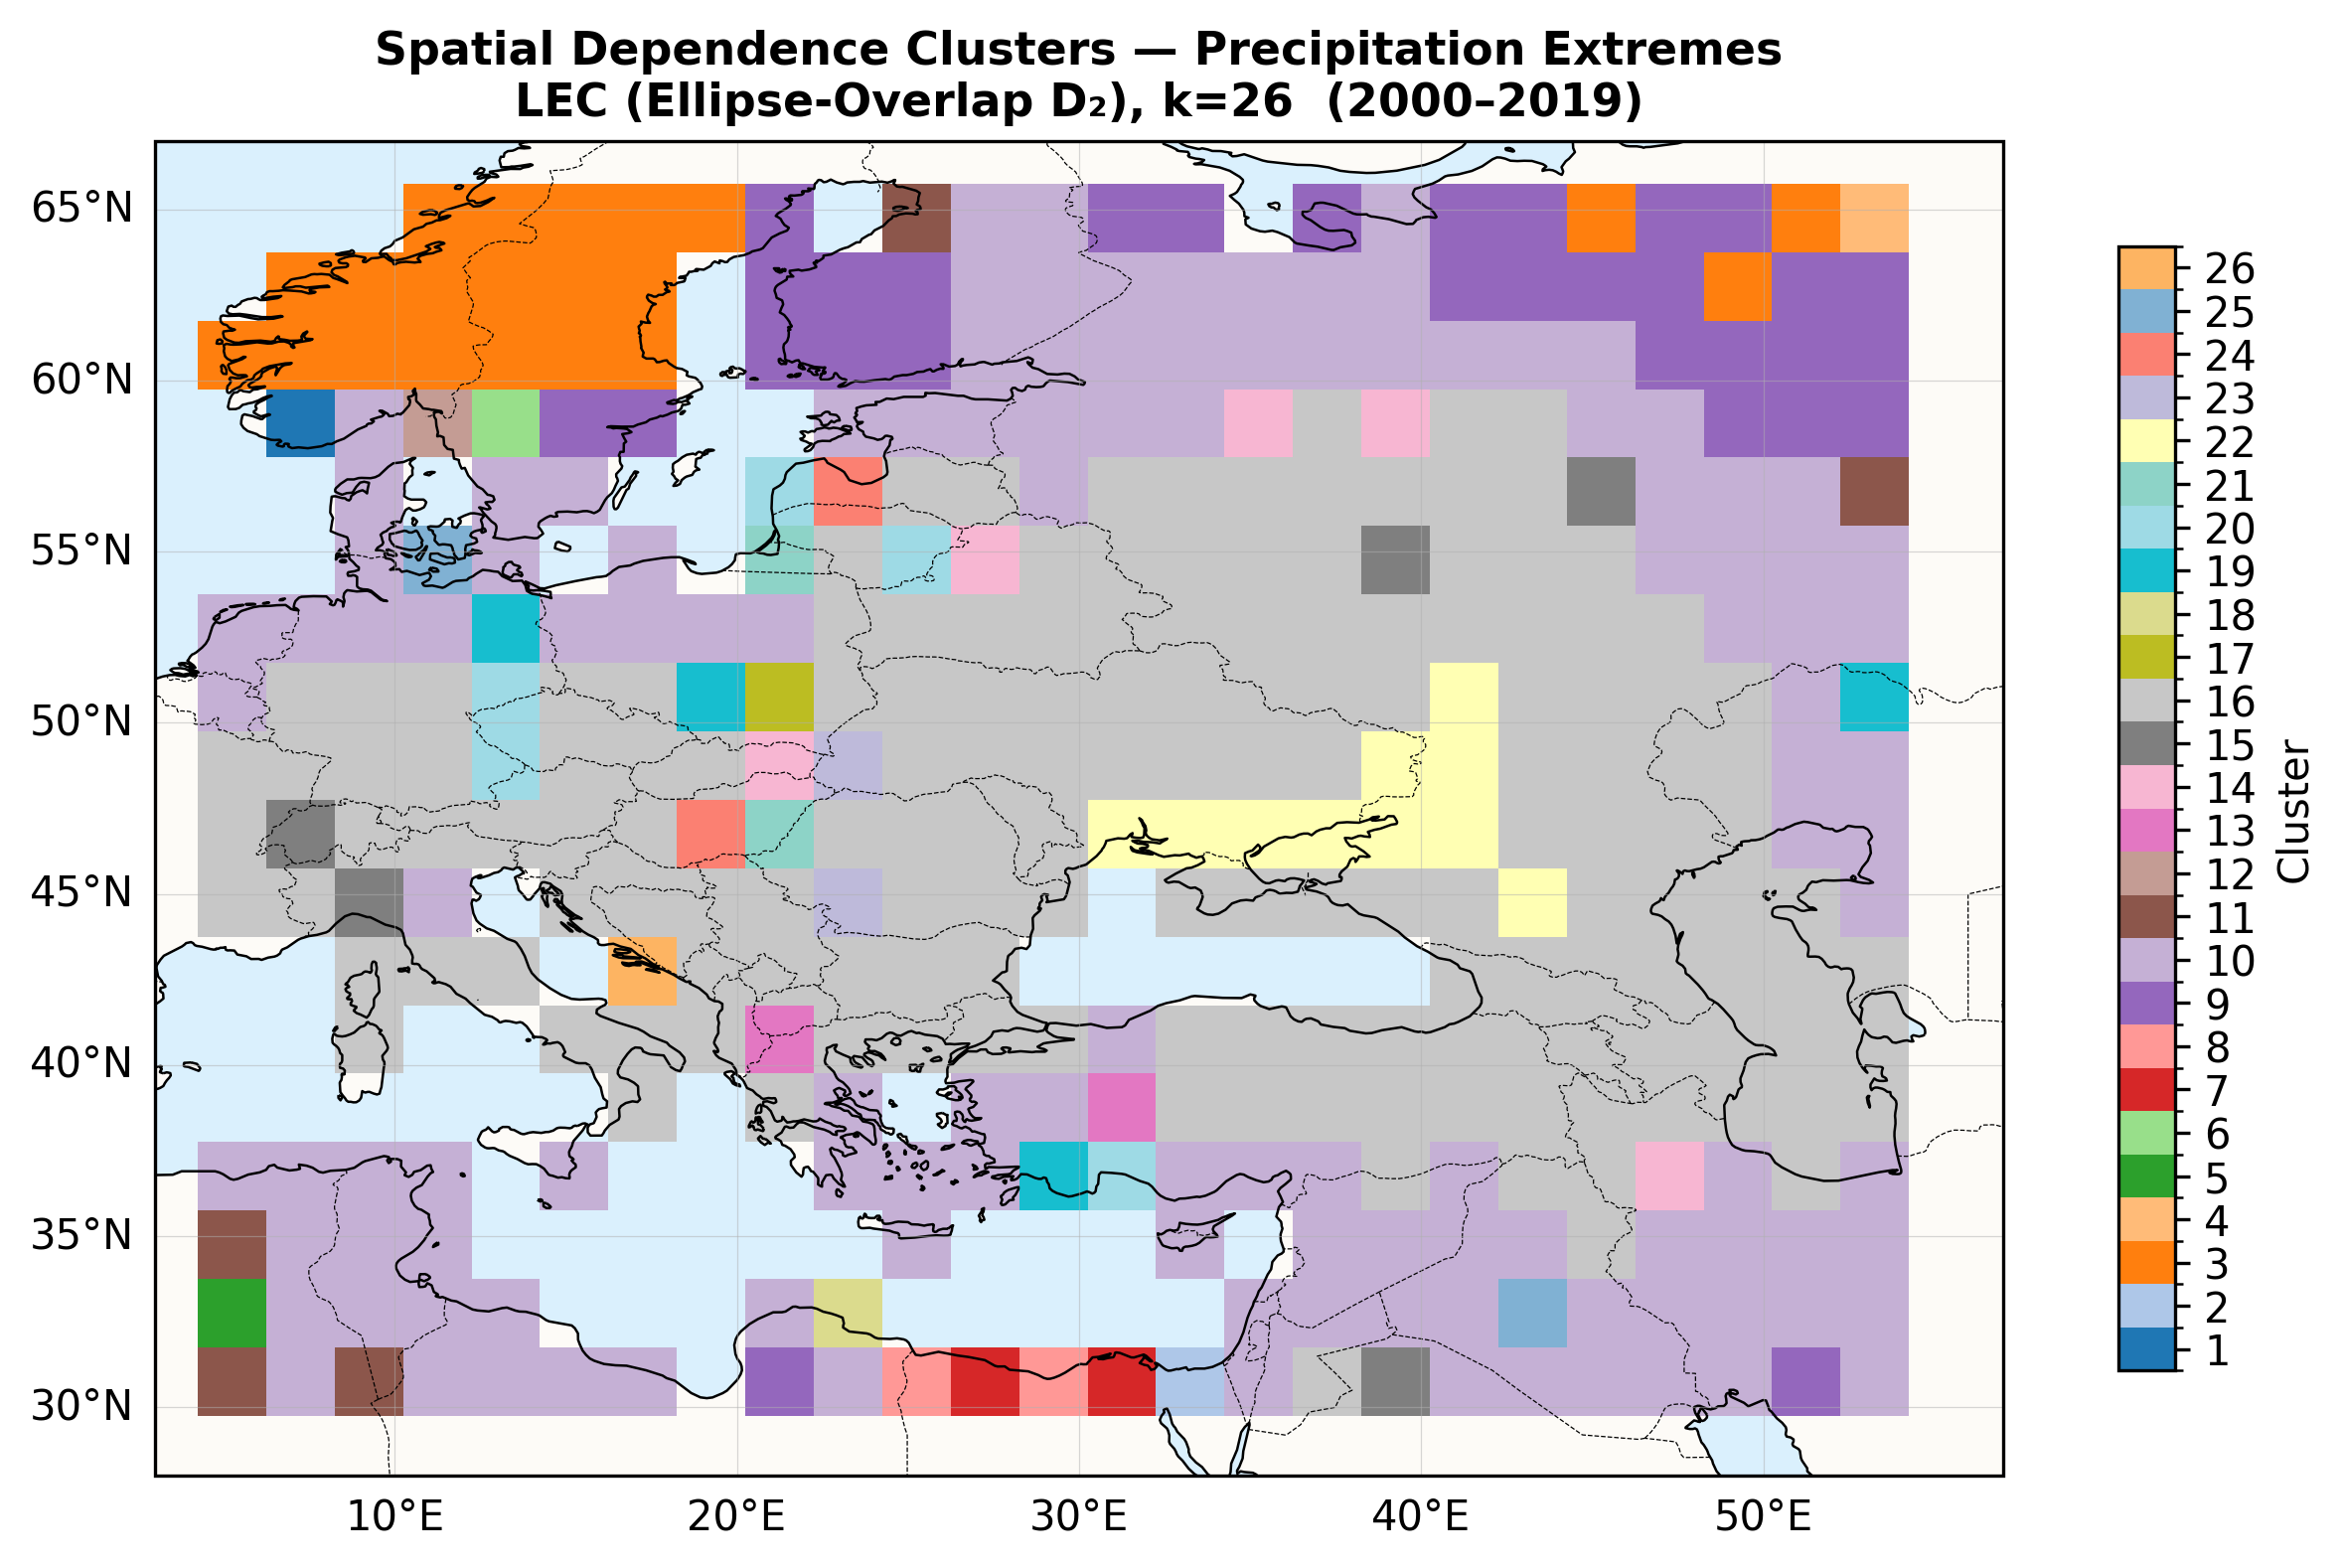
\includegraphics[width=0.95\textwidth]{figures/lec_clusters_map.png}
\caption{LEC spatial dependence clusters for CPC precipitation extremes
  (2000--2019, $k = 26$).  Clusters are determined by the ellipse-overlap
  dissimilarity $D_2$ with a 30\%-quantile threshold.  Each colour
  identifies a region of homogeneous extremal dependence structure.
  The clustering captures known climatic boundaries: the Mediterranean
  basin, Atlantic-influenced Western Europe, and continental interiors
  form distinct regions.}
\label{fig:cpc-lec-clusters}
\end{figure}

\subsubsection{GDP-weighted risk: the main result}
\label{sec:gdp-risk-result}

The key output of the pipeline is the exposure-weighted risk map.
While the per-cluster ES$_{95}$ quantifies hazard intensity on a
statistical scale, it does not distinguish between a cluster covering
an uninhabited desert and one covering a major economic centre.
By combining the hazard intensity with economic exposure at the
cell level (Equation~\ref{eq:risk-gdp}), the risk map highlights
where extreme precipitation events intersect with economic assets.

Figure~\ref{fig:cpc-gdp-risk} shows the LEC exposure-weighted risk
and Figure~\ref{fig:cpc-edc-gdp-risk} shows the EDC counterpart.
The GDP exposure layer itself is shown in Figure~\ref{fig:gdp-exposure}.

Several features are notable:
\begin{itemize}
\item Western European cells (Germany, France, Benelux) emerge as
  the highest-risk locations despite moderate hazard intensity,
  because of their high GDP density.
\item Middle Eastern and Central Asian cells with high ES$_{95}$
  (strong extremal dependence) but low GDP contribute
  negligibly to the economic risk map.
\item The cell-level formulation avoids the cluster-size bias that
  would arise from averaging GDP across entire clusters:
  a city cell within a large rural cluster correctly receives
  high risk, while neighbouring agricultural cells do not.
\end{itemize}

The total exposure-weighted risk summed across all land cells is
approximately \$6.5\,trillion (LEC) and \$4.3\,trillion (EDC),
reflecting the different cluster granularities of the two methods.

\begin{figure}[ht]
\centering
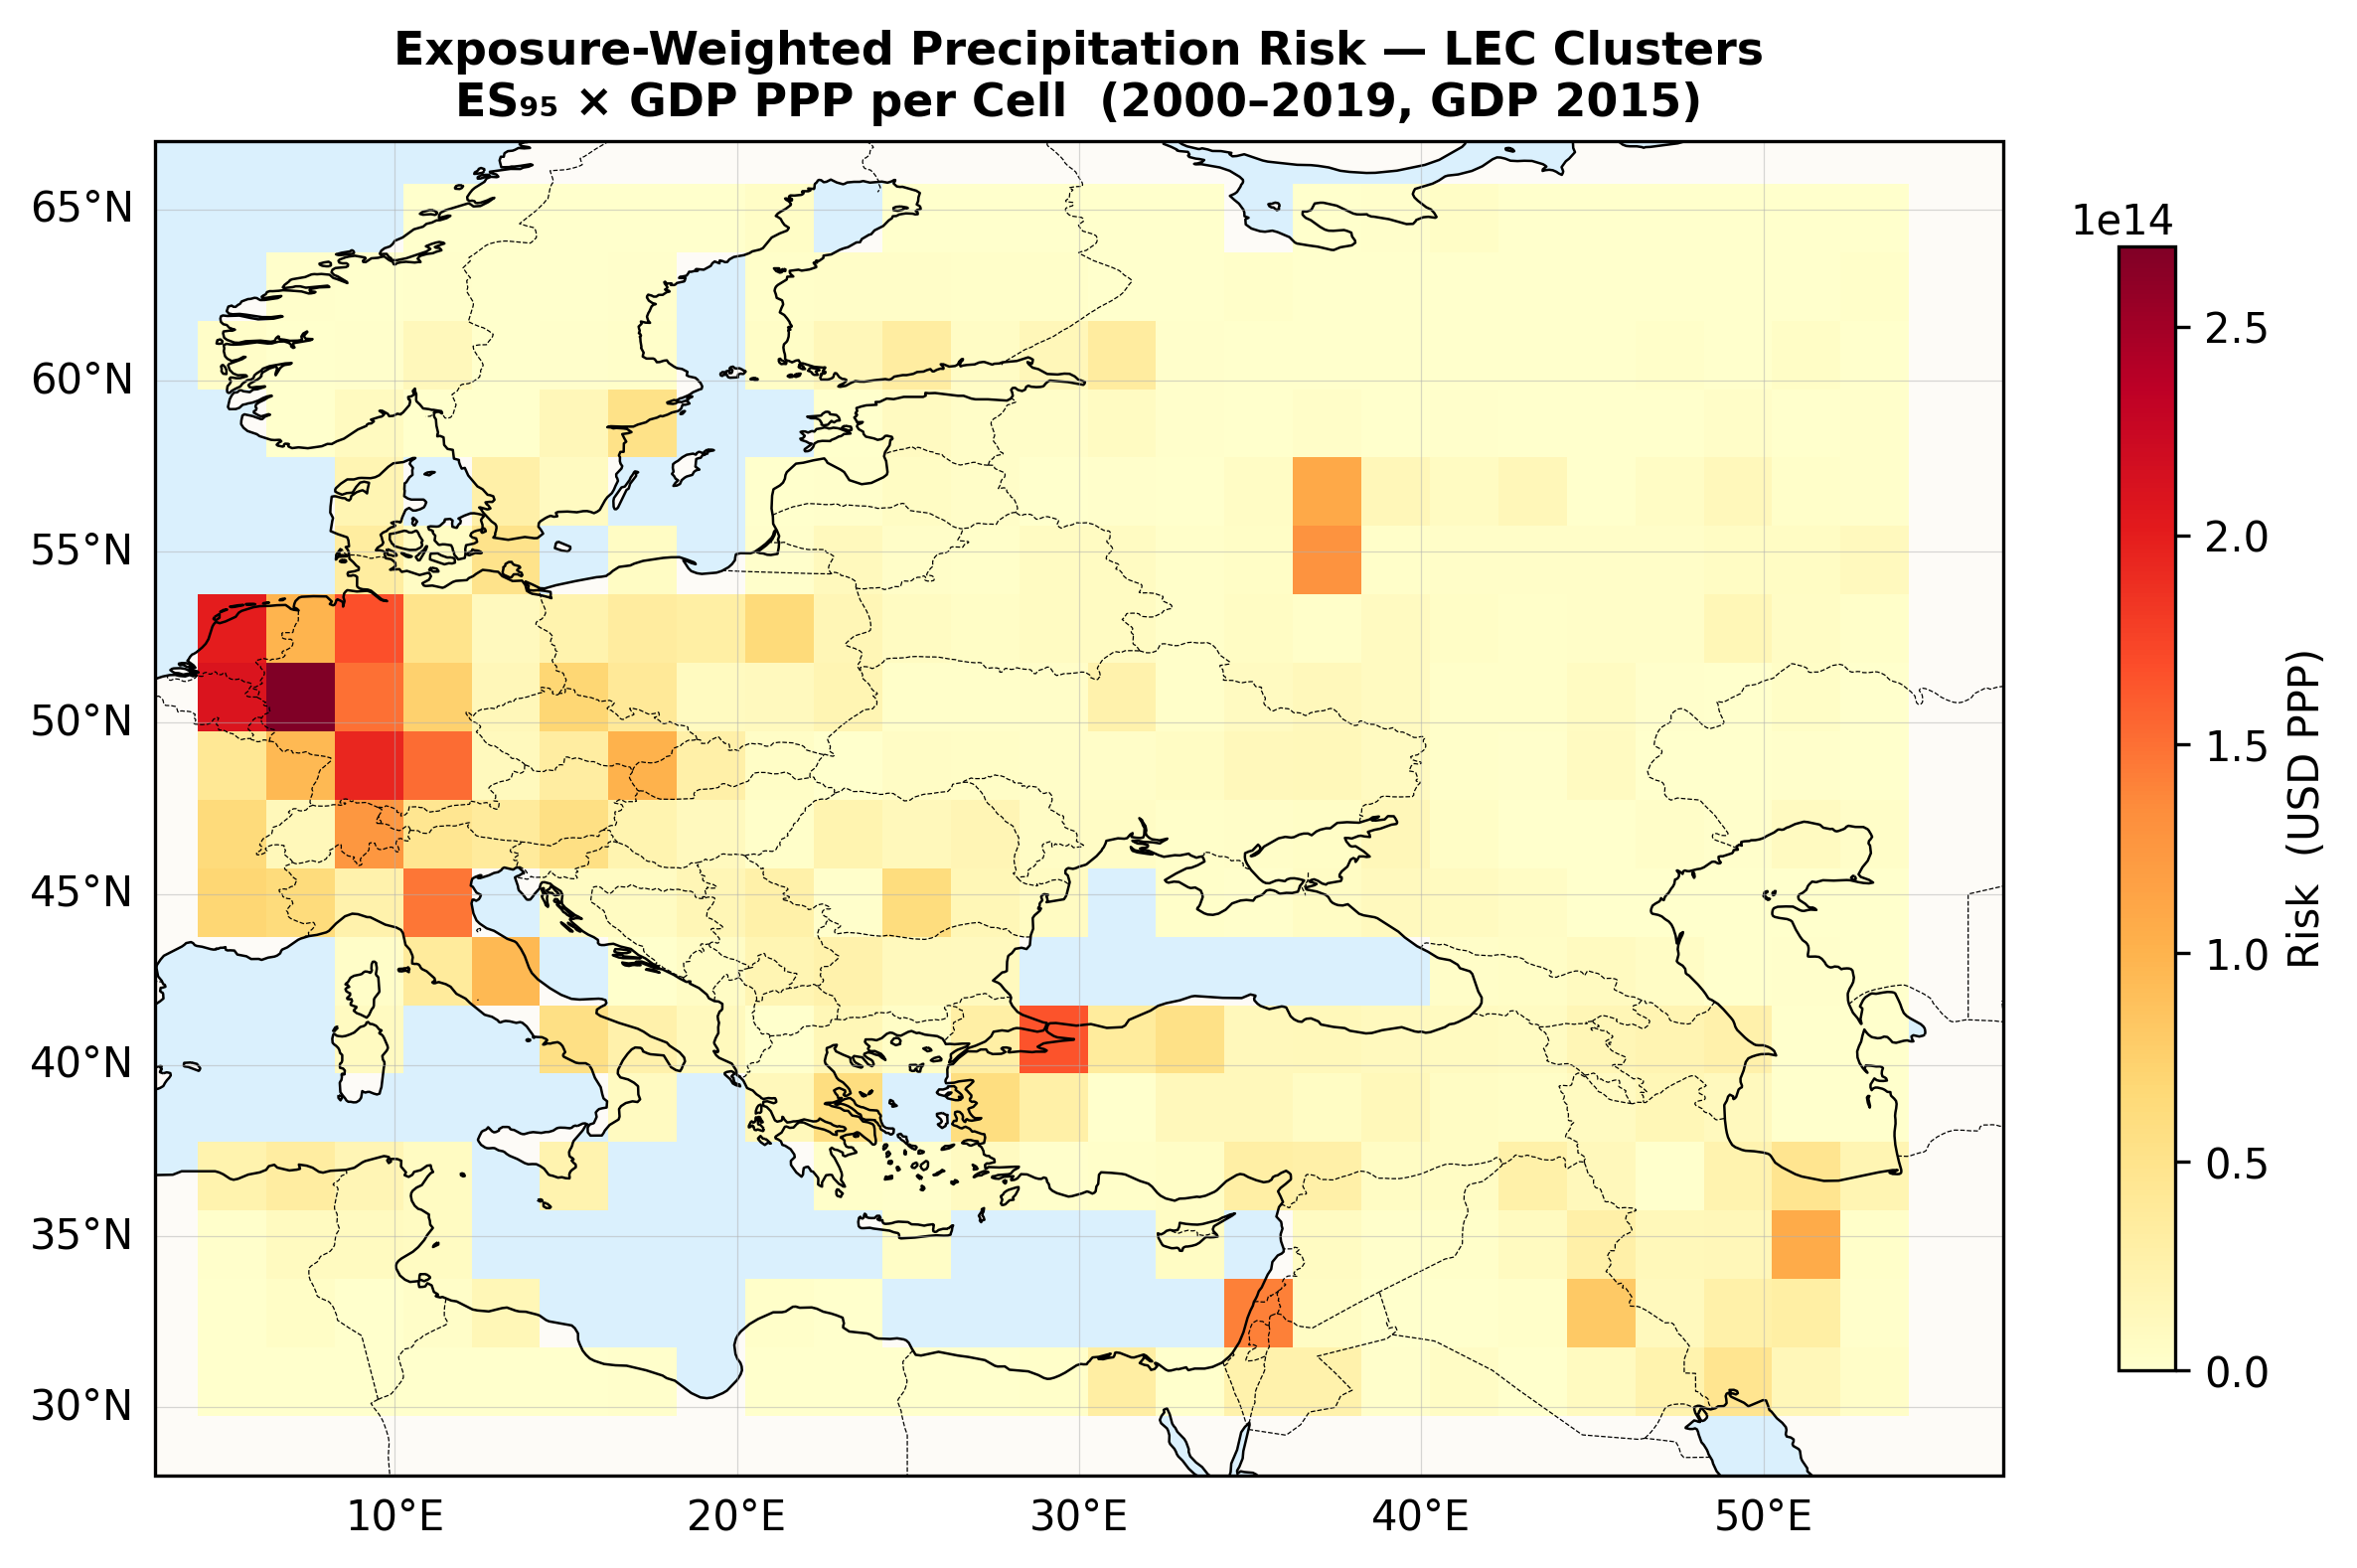
\includegraphics[width=0.95\textwidth]{figures/lec_risk_gdp_map.png}
\caption{Exposure-weighted precipitation risk (LEC clusters).
  Each cell is coloured by
  $\mathrm{Risk}(s) = \mathrm{ES}_{95}^{k(s)} \times \mathrm{GDP}(s)$.
  High-GDP areas (e.g.\ Western Europe) appear as hotspots even when
  their hazard intensity is moderate, while remote desert cells with
  high ES but negligible GDP contribute little to the risk map.
  GDP~PPP data from Kummu et al.~\cite{kummu2018}, 2015 snapshot.}
\label{fig:cpc-gdp-risk}
\end{figure}

\begin{figure}[ht]
\centering
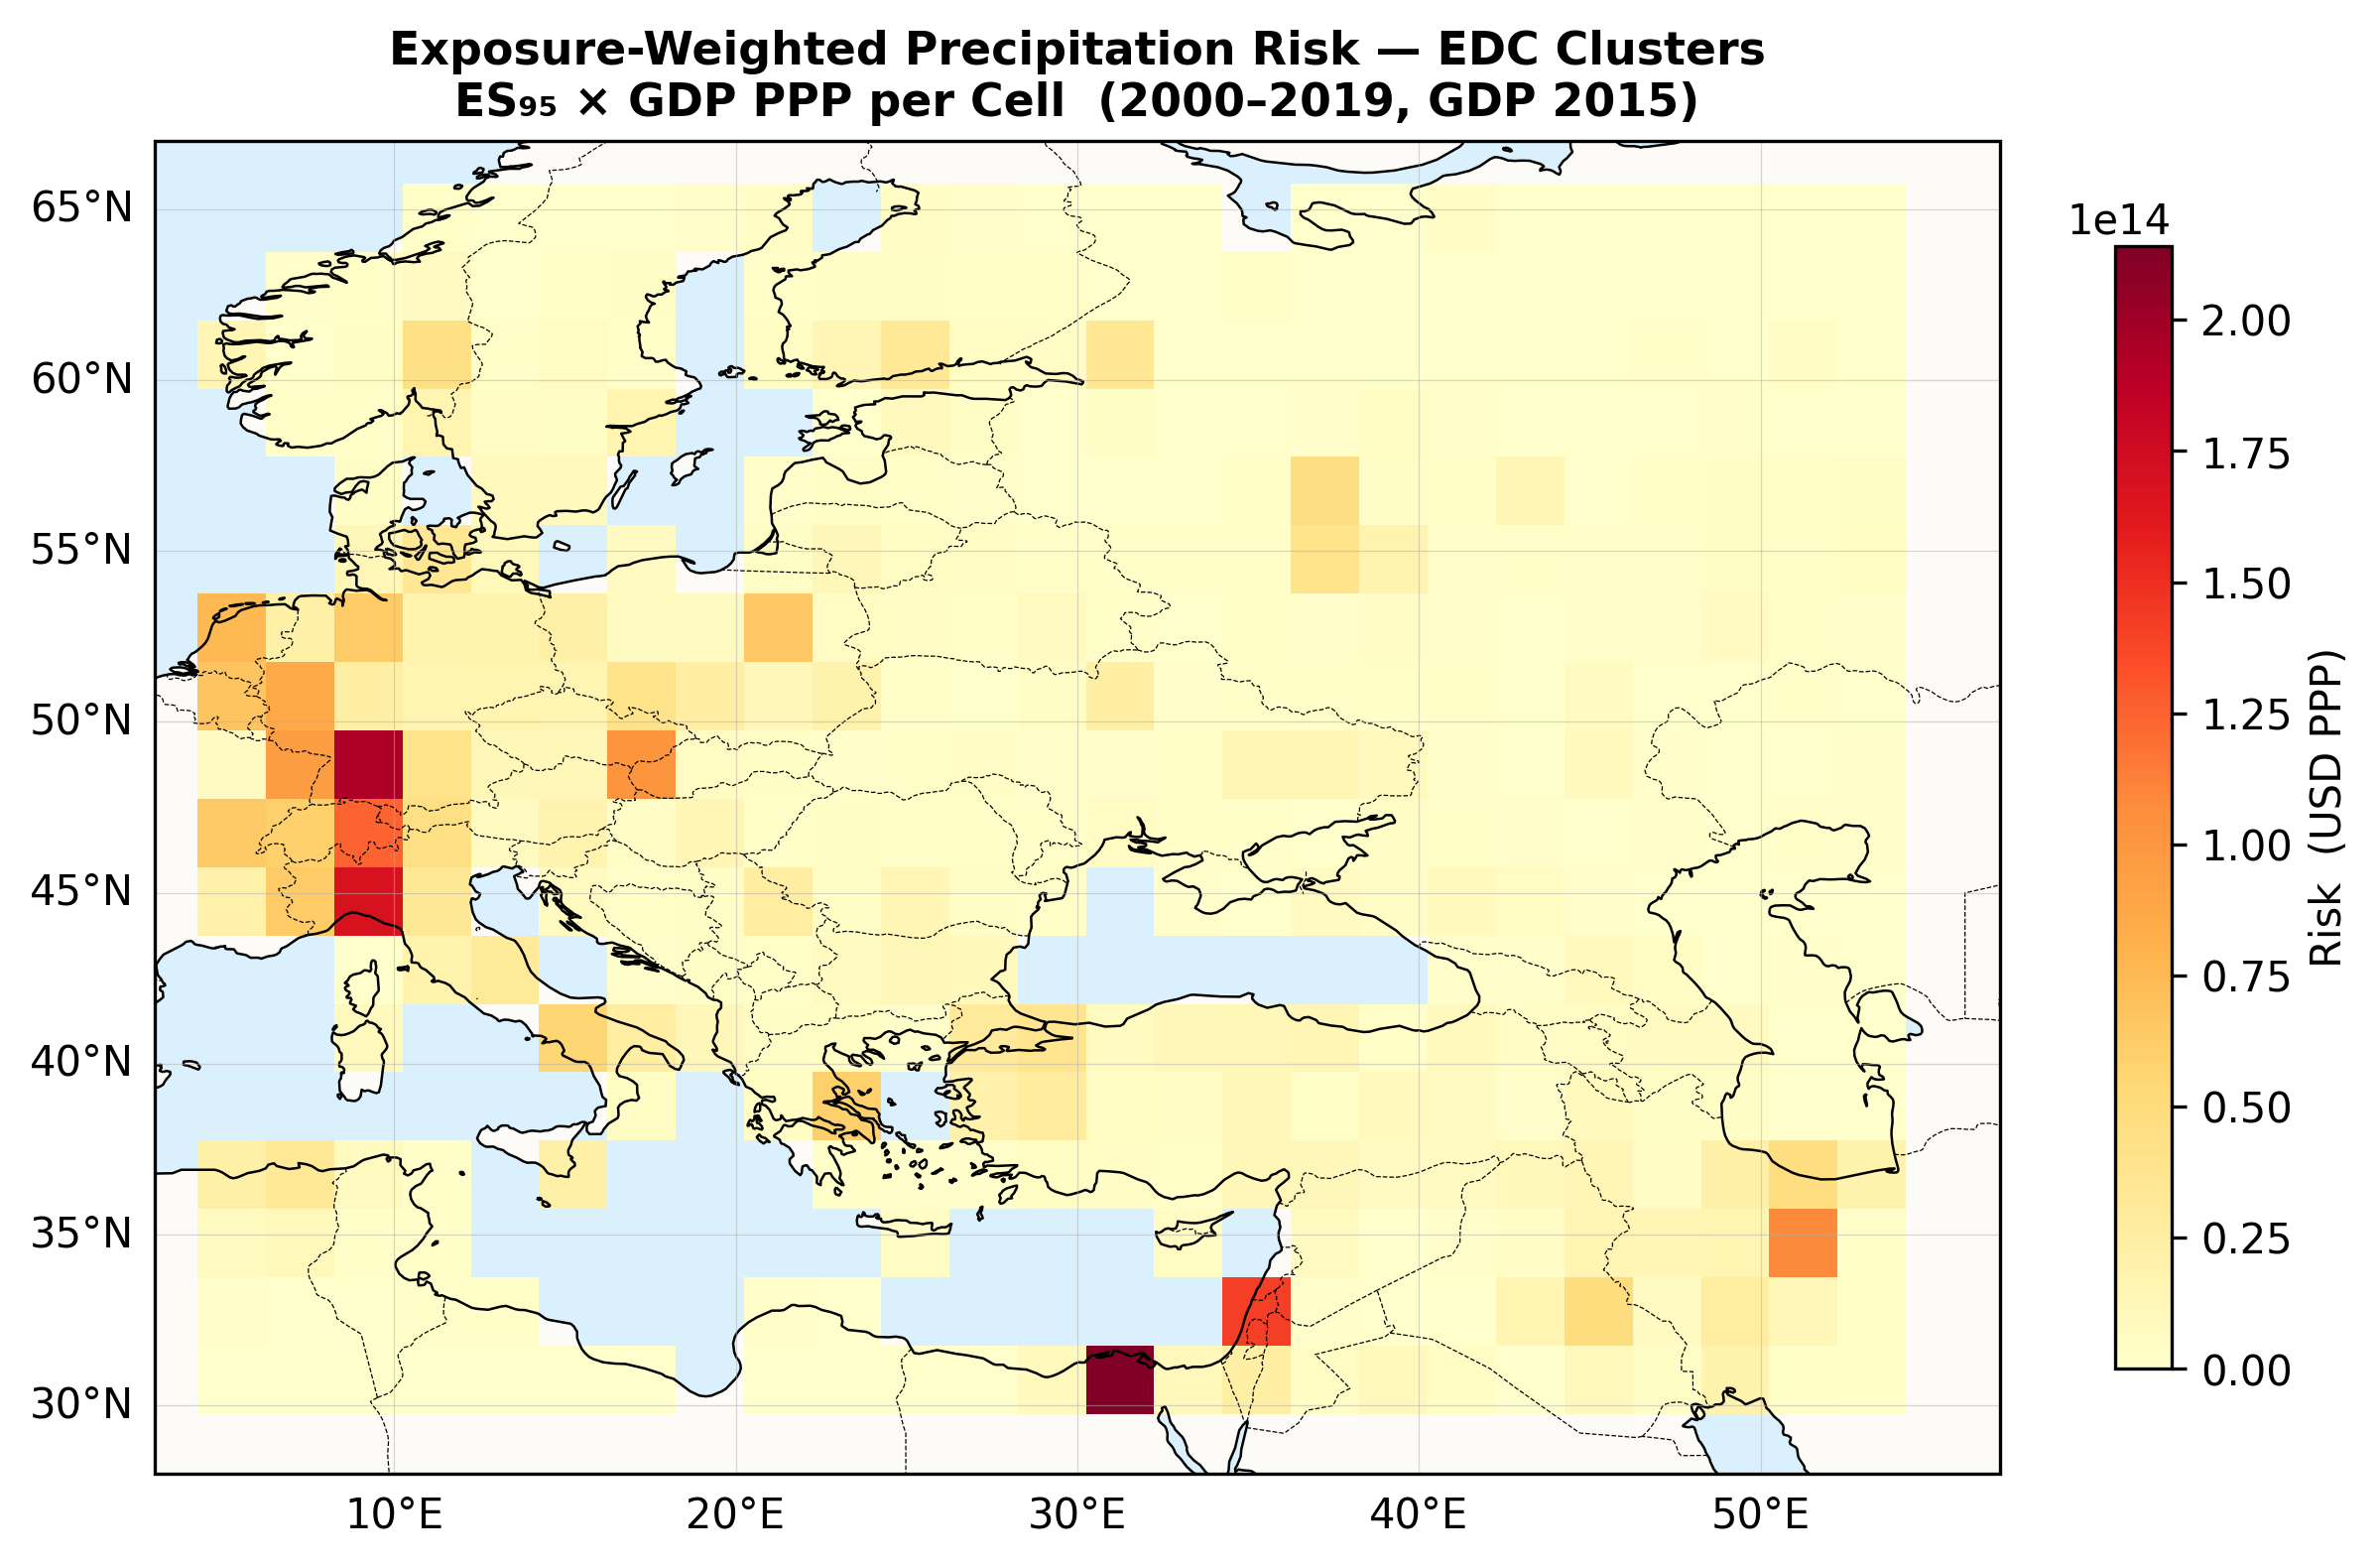
\includegraphics[width=0.95\textwidth]{figures/edc_risk_gdp_map.png}
\caption{Exposure-weighted precipitation risk (EDC clusters).
  Same formulation as Figure~\ref{fig:cpc-gdp-risk} but using
  the EDC clustering ($k = 18$, madogram dissimilarity $D_1$).
  The coarser cluster structure produces smoother risk gradients,
  with total risk approximately \$4.3\,trillion.}
\label{fig:cpc-edc-gdp-risk}
\end{figure}

\begin{figure}[ht]
\centering
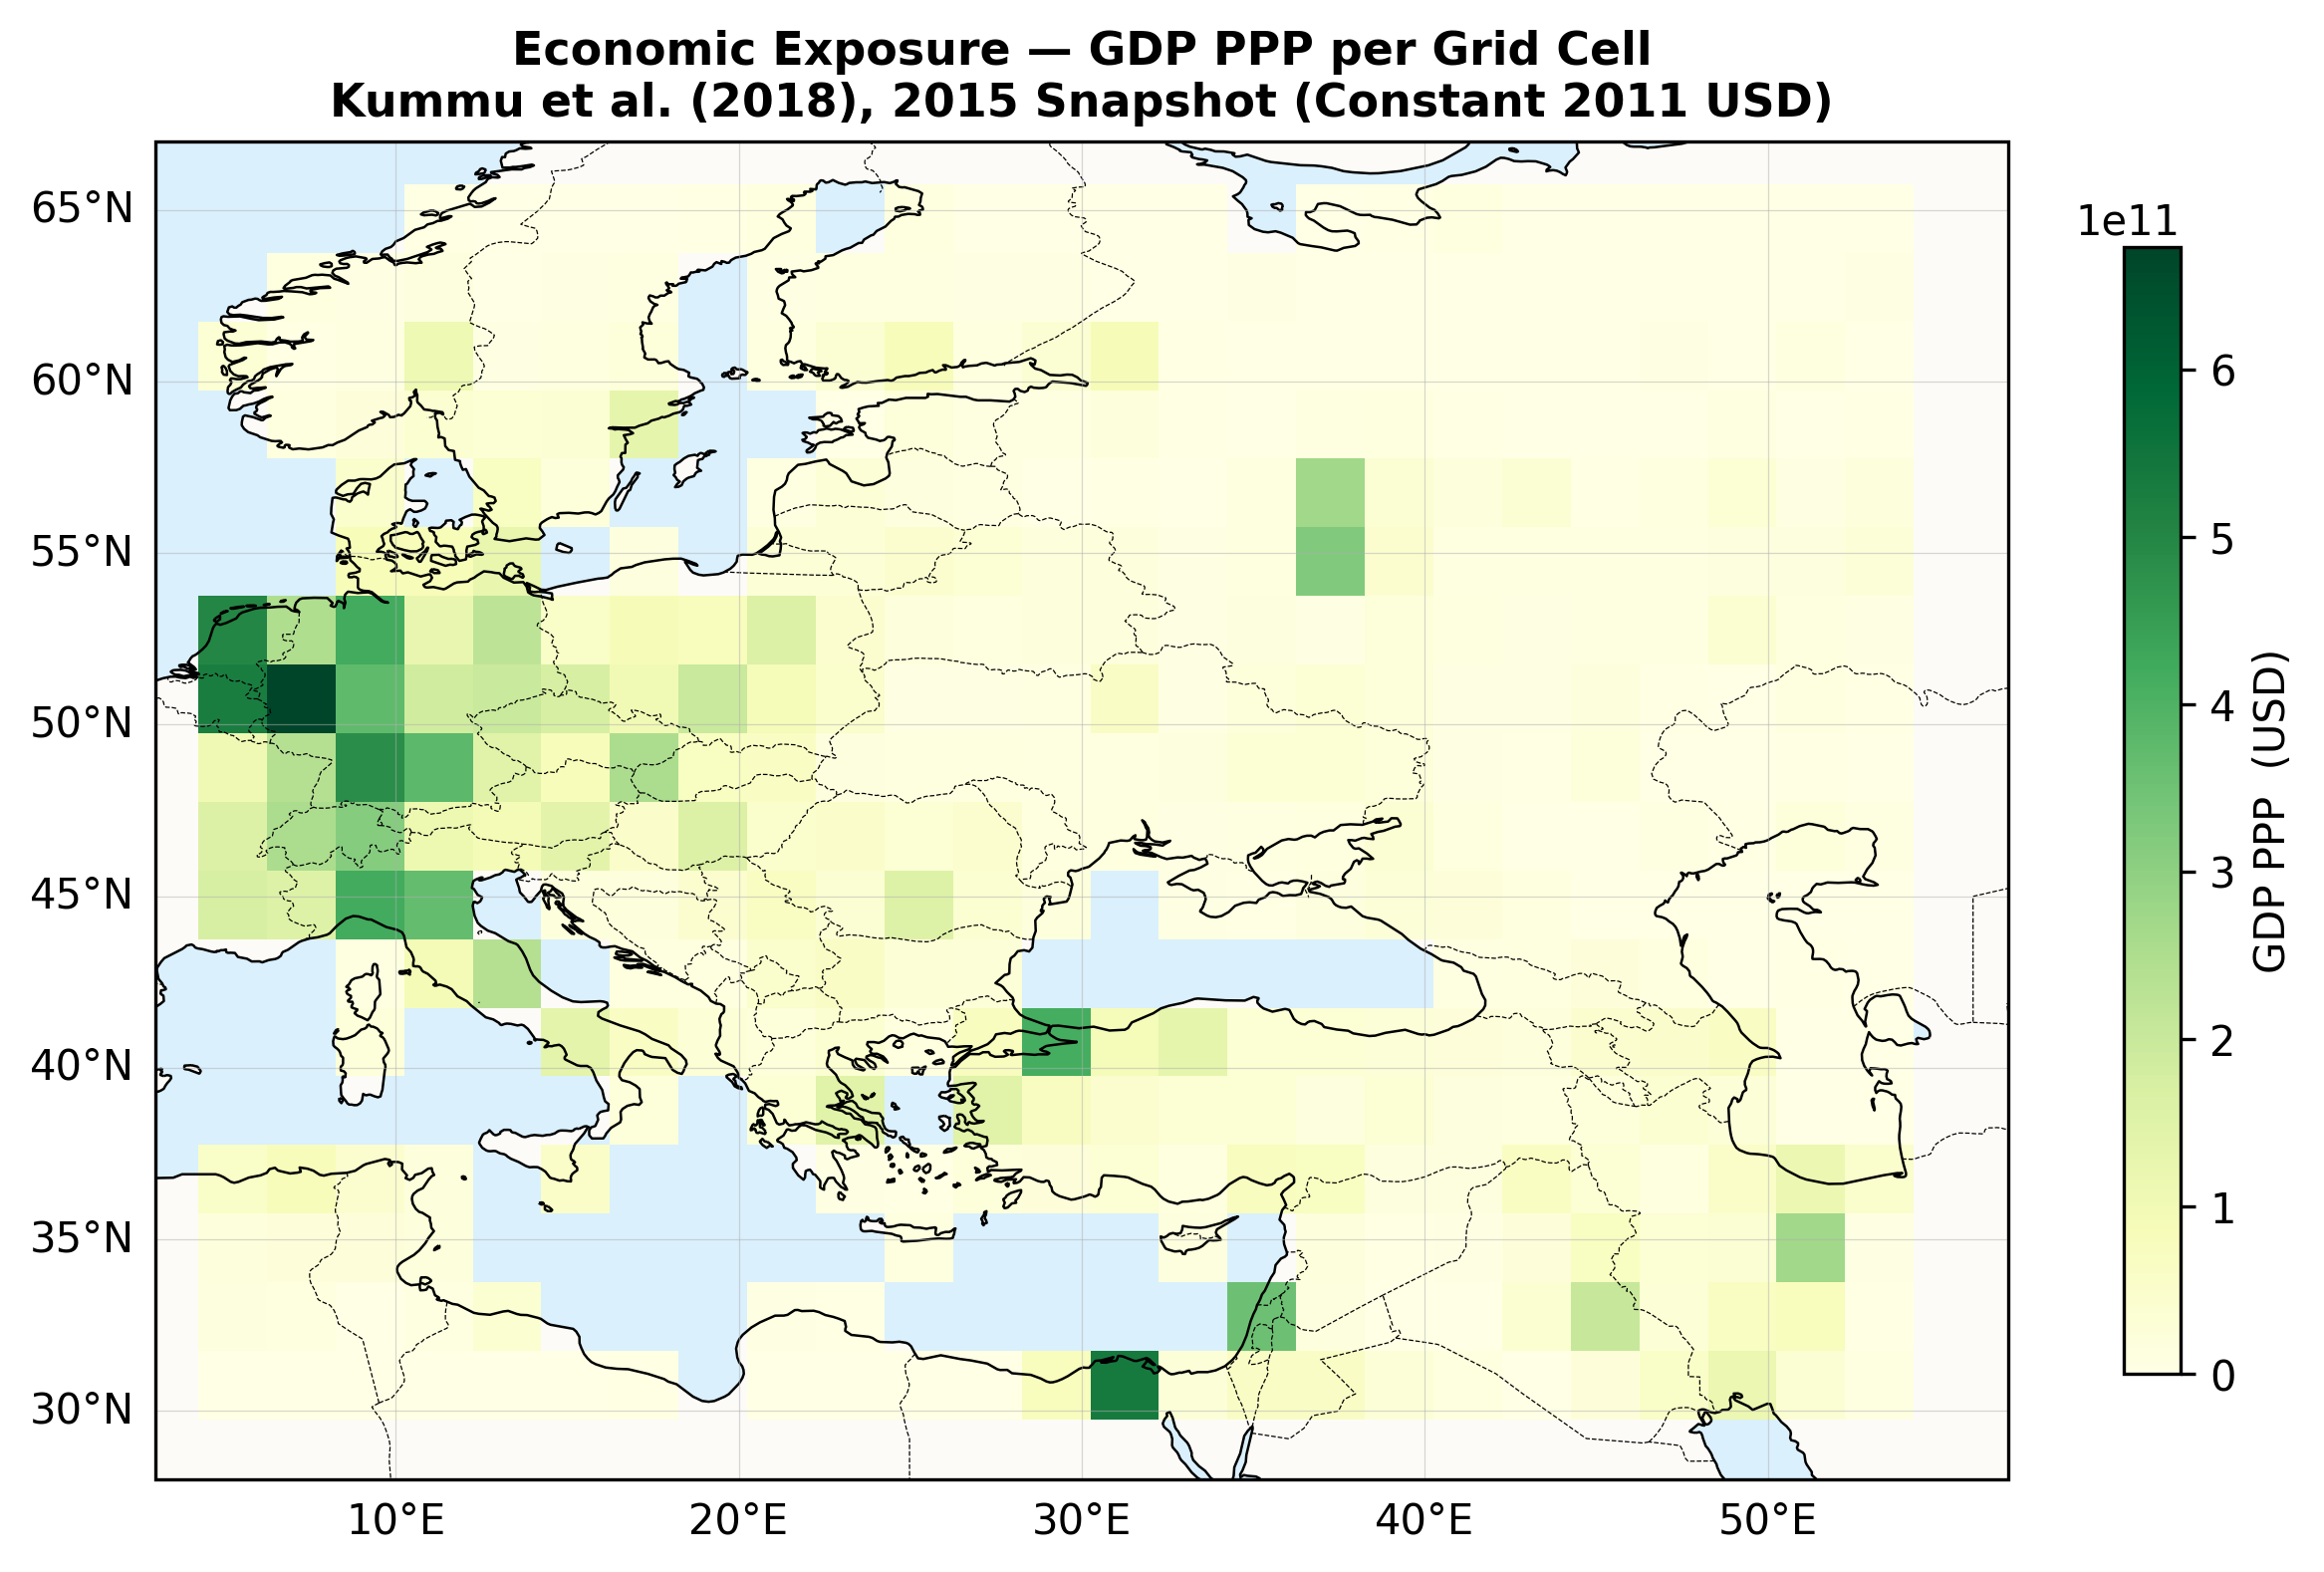
\includegraphics[width=0.95\textwidth]{figures/gdp_exposure_map.png}
\caption{Economic exposure layer: GDP~PPP per grid cell (constant 2011
  international USD), aggregated from the 5~arc-min Kummu et al.~\cite{kummu2018}
  dataset onto the $\sim$2\textdegree\ pipeline grid.
  The 2015 snapshot is used as a proxy for current economic exposure.}
\label{fig:gdp-exposure}
\end{figure}

\begin{figure}[ht]
\centering
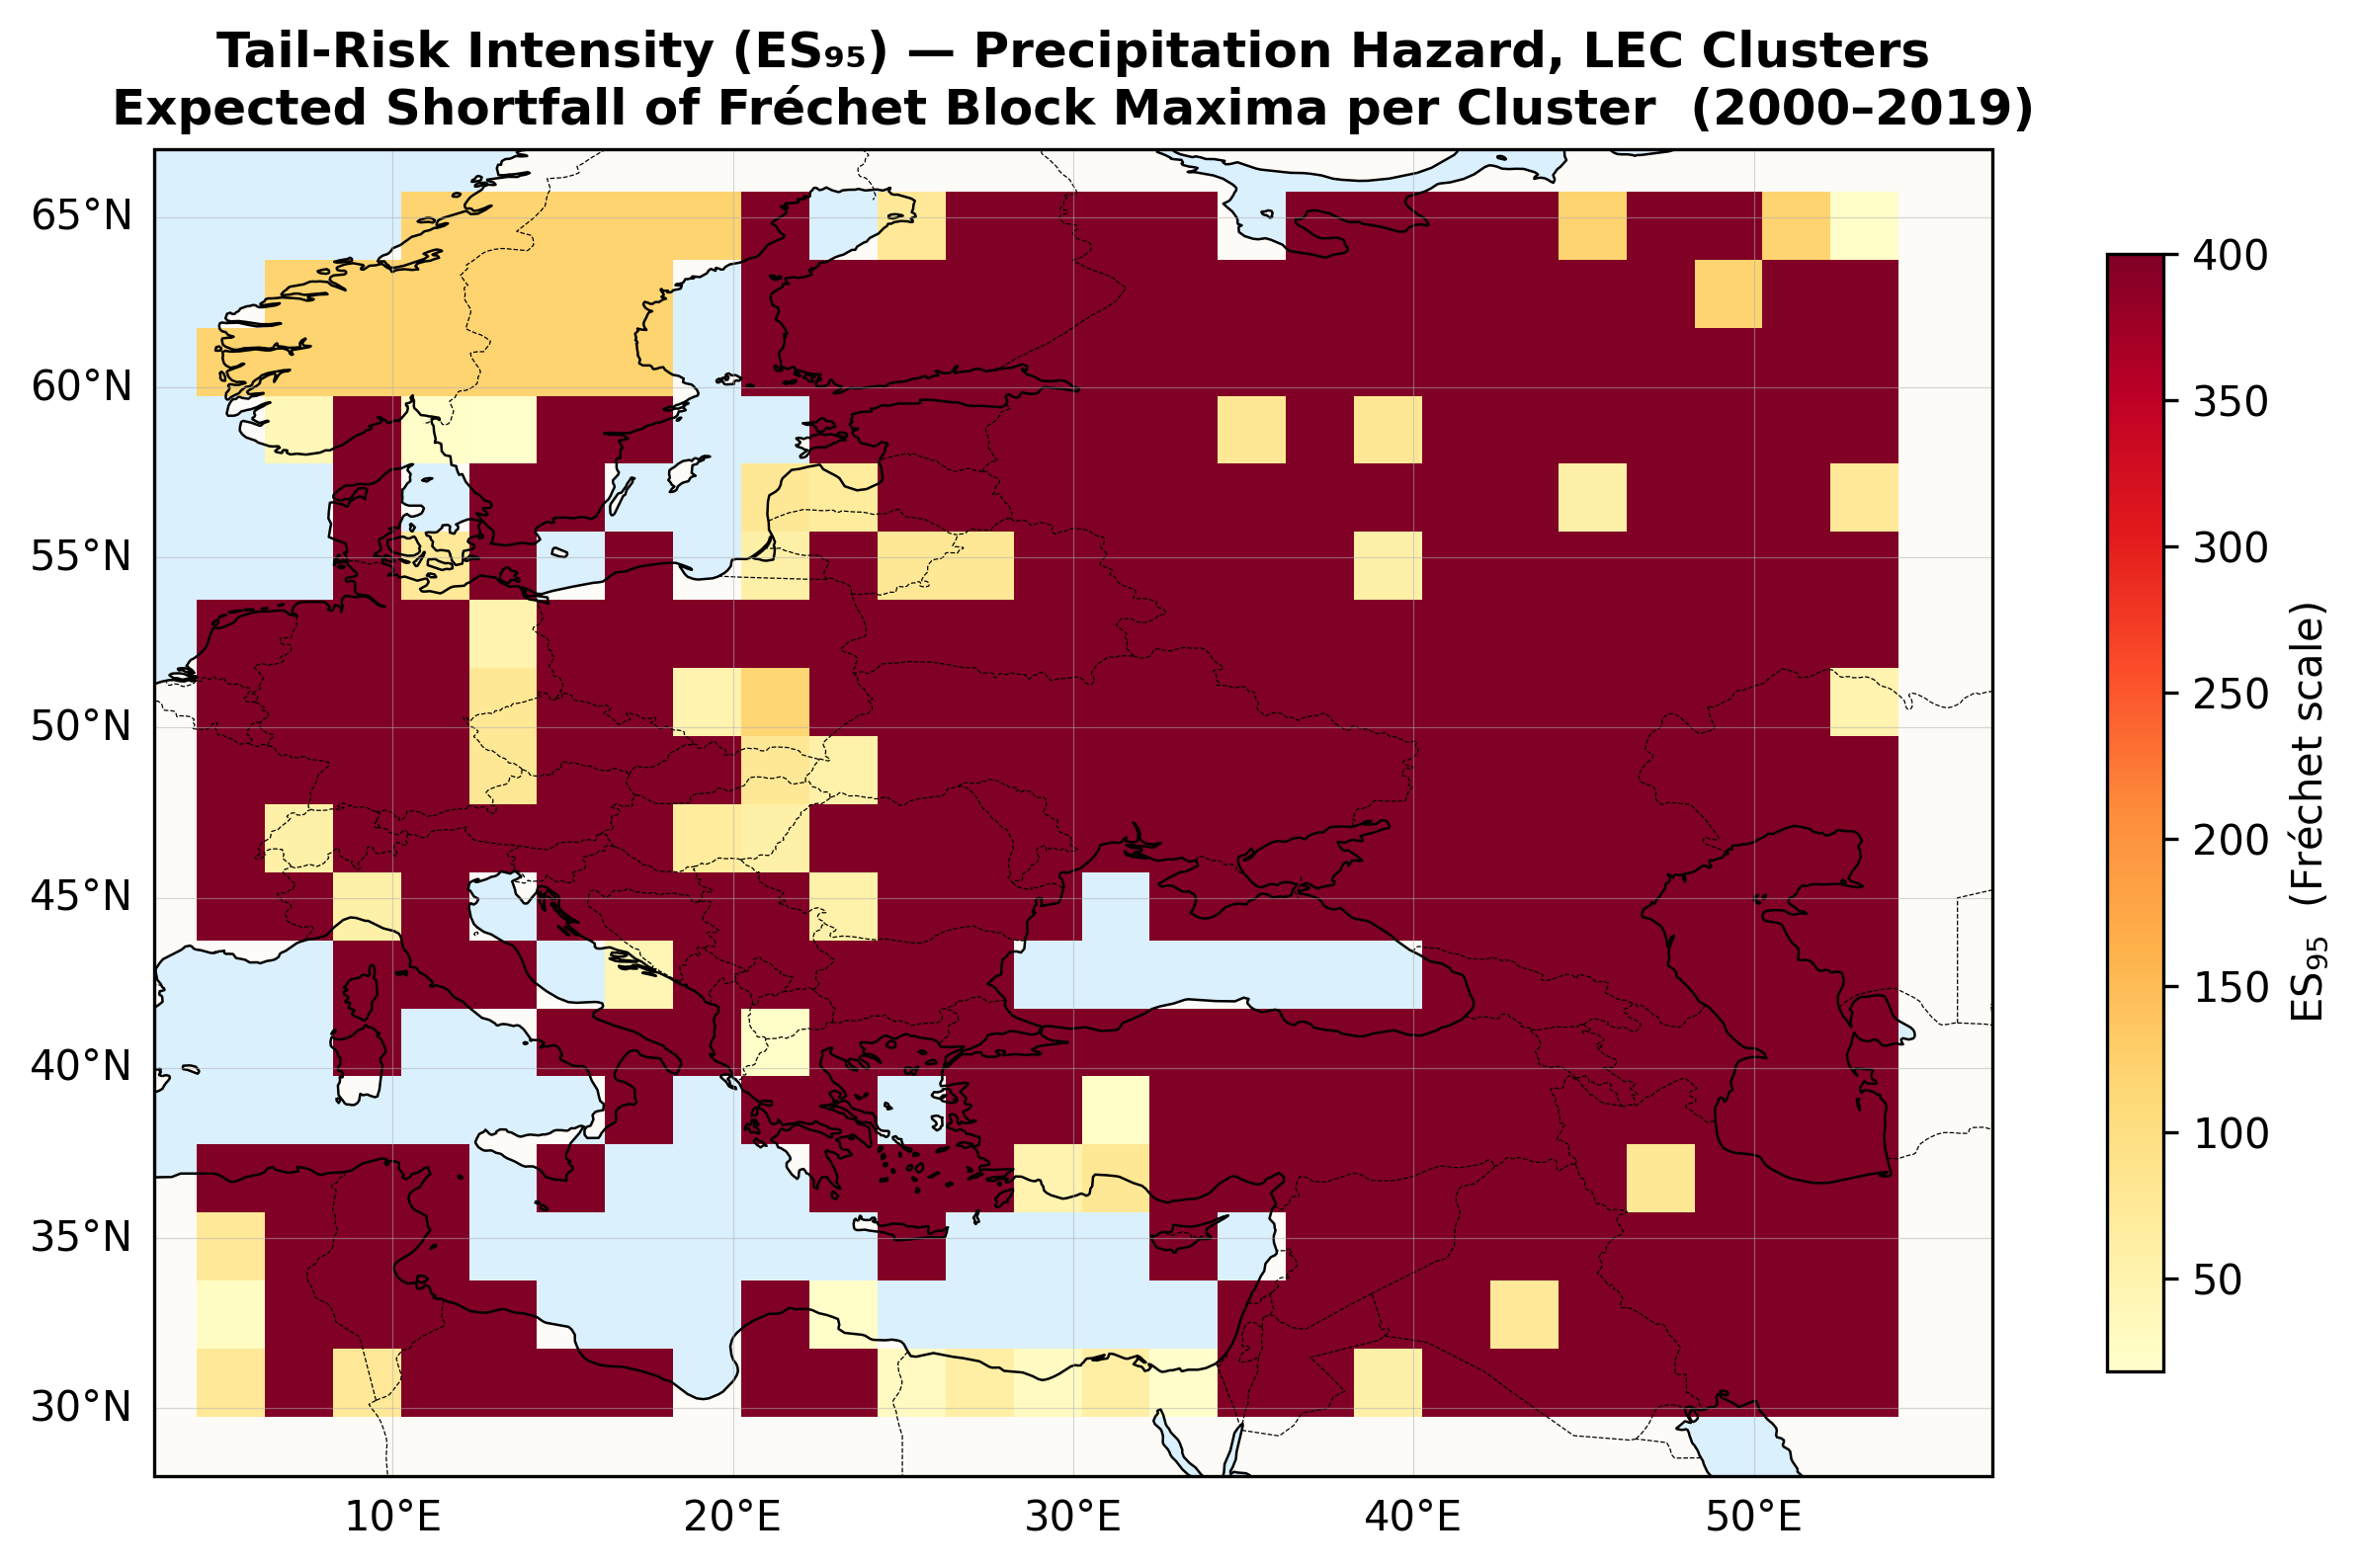
\includegraphics[width=0.95\textwidth]{figures/lec_risk_es_map.png}
\caption{Tail-risk intensity map (LEC clusters).
  Each cell inherits its cluster's ES$_{95}$ value.
  This is the hazard-only component of the risk model---high
  values indicate clusters where the joint Fréchet block maximum
  exceeds the 95th percentile by a large margin.
  Compare with Figure~\ref{fig:cpc-gdp-risk} to see how
  GDP weighting reshapes the risk landscape.}
\label{fig:cpc-lec-es}
\end{figure}

The full pipeline (data loading, estimation, clustering, GDP regridding,
and map generation) runs in approximately 100~seconds on an Apple~M2
laptop with 16\,GB RAM.

%% ============================================================
\section{Verification and validation}
\label{sec:verification}
%% ============================================================

A central concern when porting a research pipeline to a new language
is whether the port produces \emph{identical} results.
We address this rigorously with a cross-validation test suite that
executes the original R code, exports intermediate and final results,
and asserts numerical equivalence in Python.

\subsection{Methodology}

The verification proceeds in three steps:

\begin{enumerate}
\item \textbf{R reference generation.}
  A dedicated R script (\texttt{tests/generate\_r\_reference.R},
  478~lines) sources the original R functions
  (\texttt{r\_code/functions.R} and \texttt{r\_code/parameters.R}),
  executes every pipeline stage on the ``stripes'' preset
  ($10 \times 10$ grid, $\nu = 5$, $\alpha = 1$, 10~simulations,
  seed~42), and exports 34~CSV files to
  \texttt{tests/reference\_data/}.
  These files contain: grid coordinates, axis vectors,
  index-conversion test cases, parameter matrices,
  covariance function evaluations (150+ stationary cases, 5~non-stationary cases,
  18 extremal-coefficient conversion cases),
  pairwise density and $\partial t/\partial\text{diff}$ evaluations,
  full $100 \times 100$ covariance matrices (stationary and non-stationary),
  non-stationary simulation output,
  madogram and extremal-coefficient matrices,
  raw and smoothed local estimates,
  ellipse dissimilarity matrix,
  hierarchical clustering details (merge partners, heights, leaf order)
  for both LEC and EDC methods,
  cluster assignments, and per-cluster log-likelihoods.

\item \textbf{Cross-validation tests.}
  A Python test module (\texttt{tests/test\_r\_cross\_validation.py},
  775~lines) loads every reference CSV and compares the output of the
  corresponding Python function against the R reference.
  R uses column-major (Fortran-order) flattening of the 2-D grid;
  the Python port now uses the same convention throughout
  (\texttt{grid\_number}, \texttt{number\_grid},
  \texttt{X\_flat}, \texttt{Y\_flat}, and the flat reshape
  in \texttt{c\_extrcoeff\_matrix} all use Fortran order),
  so index comparisons are direct.

\item \textbf{R-parity fix tests.}
  A second test module (\texttt{tests/test\_r\_parity\_fixes.py},
  22~tests) verifies the five algorithmic fixes that bring the
  Python implementation into exact alignment with R:
  column-major grid indexing, parameter rescaling (\texttt{parscale}),
  gamma-wrapping retry at the $\pm\pi/2$ boundary,
  boundary-proximity retry for the local optimiser,
  and average log-likelihood computation in
  \texttt{calc\_estimates\_in\_clusters}.

\item \textbf{Continuous integration.}
  The 50~cross-validation and R-parity tests are integrated into
  the project's \texttt{pytest} suite (105~tests total) and run on
  every commit.
\end{enumerate}

\subsection{Results}

Table~\ref{tab:verification} summarises the cross-validation results
across all pipeline components.  Every test passes.

\begin{table}[ht]
\caption{Cross-validation results: Python vs.\ original R code.
  All 50 tests pass (28~cross-validation + 22~R-parity fix tests).
  Tolerance column shows the maximum absolute
  difference permitted (``exact'' means partition identity is checked
  by verifying that every pair of grid points is assigned to the
  same or different cluster in both implementations).}
\label{tab:verification}
\centering
\footnotesize
\begin{tabular}{@{}p{3.6cm}lrl@{}}
\toprule
\textbf{Component} & \textbf{Tests} & \textbf{Tolerance} & \textbf{Result} \\
\midrule
Grid axes \& coordinates     & 2  & $10^{-12}$ & pass \\
Index conversions             & 3  & exact (0/1)& pass \\
Parameter matrices $(a,b,\gamma)$ & 1 & $10^{-10}$ & pass \\
\texttt{cov\_fkt\_2d} (150+ cases)& 2 & $10^{-12}$ & pass \\
\texttt{cov\_fkt\_2d\_nonstat2}   & 1 & $10^{-10}$ & pass \\
\texttt{cov\_to\_ec}              & 1 & $10^{-10}$ & pass \\
\texttt{ec\_to\_cov}$^{\dagger}$  & 1 & $10^{-4}$  & pass \\
$\partial t$-density derivative   & 1 & $10^{-12}$ & pass \\
Pairwise density summand      & 1  & $10^{-8}$  & pass \\
Covariance matrix (stat.)     & 1  & $10^{-12}$ & pass \\
Covariance matrix (non-stat.) & 1  & $10^{-10}$ & pass \\
Madogram matrix               & 1  & $10^{-12}$ & pass \\
Extremal coeff.\ matrix       & 1  & $10^{-12}$ & pass \\
Ellipse dissimilarity         & 1  & $0.5$      & pass \\
Smoothing ($a$, $b$)          & 1  & $10^{-8}$  & pass \\
Smoothing ($\gamma$, circular)& 1  & $10^{-6}$  & pass \\
LEC cluster count \& heights  & 2  & $10^{-6}$  & pass \\
LEC partition equivalence     & 1  & exact      & pass \\
EDC cluster count$^{\ddagger}$& 1  & $\pm 1$    & pass \\
EDC merge heights$^{\ddagger}$& 1  & $5 \times 10^{-3}$ & pass \\
EDC partition similarity      & 1  & $\geq$95\% & pass \\
Log-likelihood in clusters    & 1  & $10^{-4}$  & pass \\
End-to-end EDC pipeline       & 1  & $\pm 1$ $k$& pass \\
\midrule
\multicolumn{4}{@{}l}{\itshape R-parity fix tests
  (\texttt{test\_r\_parity\_fixes.py})} \\[2pt]
Column-major grid indexing    & 5  & exact      & pass \\
Fortran-order \texttt{X\_flat}/\texttt{Y\_flat} & 4 & $10^{-12}$ & pass \\
Parscale (local + global)     & 2  & in-bounds  & pass \\
Gamma-wrapping retry          & 2  & finite     & pass \\
Boundary-proximity retry      & 3  & finite     & pass \\
Avg.\ LLH in clusters (col.~4) & 3 & finite     & pass \\
Column-major cluster coords   & 1  & finite     & pass \\
Integration (local + smooth)  & 2  & finite     & pass \\
\midrule
\textbf{Total}                & \textbf{50} & & \textbf{50 pass} \\
\bottomrule
\end{tabular}

\smallskip
\raggedright\scriptsize
$^{\dagger}$\,\texttt{ec\_to\_cov} inverts \texttt{cov\_to\_ec} via root-finding.
  The $2.6 \times 10^{-5}$ discrepancy at $\nu = 1$ arises from
  algorithmic differences between R's \texttt{pt()} and SciPy's
  \texttt{t.cdf()} for Student-$t$ CDF evaluation.
  At $\nu \geq 5$ (the setting used in practice), the difference
  is below $10^{-10}$.

$^{\ddagger}$\,The EDC (Saunders) method uses rank-based
  madogram distances that produce many tied values when only
  $n_{\mathrm{sim}} = 10$ simulations are used.
  UPGMA tie-breaking differs between R's \texttt{hclust()} and
  SciPy's \texttt{linkage()}, causing merge heights to diverge
  by up to one rank step ($\sim$0.005) and cluster counts to differ by $\pm 1$.
  With the 20+ simulations used in practice, ties are rare and
  both implementations converge to identical partitions.
  The LEC method (continuous ellipse distances, no ties)
  matches exactly.
\end{table}

\subsection{Discussion of known differences}

The verification confirms that the Python port is a faithful reproduction
of the R code for all practical purposes.
Three categories of difference are documented:

\begin{enumerate}
\item \textbf{Student-$t$ CDF implementation} (affects \texttt{ec\_to\_cov} only):
  R and SciPy use different internal algorithms for the Student-$t$
  cumulative distribution function.  For $\nu = 1$ and $\rho$ close to~1,
  this produces a discrepancy of $\sim$$2.6 \times 10^{-5}$ in the
  recovered covariance.
  At the degrees of freedom used in practice ($\nu \geq 5$), the
  difference is below $10^{-10}$ and has no effect on downstream results.

\item \textbf{UPGMA tie-breaking} (affects EDC/Saunders clustering only):
  When the pairwise dissimilarity matrix contains many tied distances
  (common with rank-based madogram on few simulations), the
  UPGMA merge order depends on implementation-specific tie-breaking.
  R's \texttt{hclust()} and SciPy's \texttt{linkage()} make
  different choices, producing slightly different dendrograms
  and hence $\pm 1$ cluster.
  The LEC method uses continuous Jaccard-like ellipse distances
  that have no ties, and its clustering matches R exactly.

\item \textbf{Column-major vs.\ row-major ordering} (resolved):
  R's \texttt{as.vector()} flattens matrices in column-major (Fortran)
  order; NumPy defaults to row-major (C) order.
  In earlier versions of \texttt{weatherisk}, this caused index
  mismatches in the madogram matrix, extremal-coefficient matrix,
  and local estimation coordinate lookups.
  This has been fully resolved: all grid-index functions
  (\texttt{grid\_number}, \texttt{number\_grid}, \texttt{koord\_num},
  \texttt{number\_koord}), the flattened coordinate vectors
  (\texttt{X\_flat}, \texttt{Y\_flat}), and the reshape in
  \texttt{c\_extrcoeff\_matrix} now use Fortran order,
  matching R exactly.
\end{enumerate}

In addition to resolving the index-ordering issue, five further
algorithmic fixes were applied to match R's optimisation heuristics:

\begin{enumerate}
\item \textbf{Parameter rescaling (parscale)}:
  R's \texttt{optim()} with \texttt{control=list(parscale=p)}
  rescales each optimisation variable by \texttt{(upper$-$lower)/100}.
  Both \texttt{pairwise\_density\_optim} and
  \texttt{pairwise\_density\_optim\_local} now apply the same
  rescaling before calling L-BFGS-B.

\item \textbf{Gamma-wrapping retry}:
  When the estimated rotation $\gamma$ hits the $\pm\pi/2$ boundary,
  the optimiser re-starts with $-\gamma$ (flipping the sign),
  matching R's \texttt{if(abs(abs(par[3])-pi/2)<1e-10)} guard.

\item \textbf{Boundary-proximity retry} (local optimiser only):
  If any parameter lands within 0.01 of its bounds, the local
  optimiser draws the next Latin Hypercube start point and
  re-tries, up to 5~extra attempts.
  This matches R's \texttt{while(near\_boundary \&\& i < length(starts))} loop.

\item \textbf{Average log-likelihood in clusters}:
  \texttt{calc\_estimates\_in\_clusters} now calls
  \texttt{llh\_in\_cluster(average=True)} and stores the result
  in column~4, matching R's \texttt{estimates\_in\_clusters[i,5]}.
\end{enumerate}

None of the remaining differences affect scientifically meaningful results:
all covariance values, density evaluations, extremal coefficients,
smoothed estimates, dissimilarity matrices, and LEC cluster assignments
are numerically identical (to machine precision or better) between
the R and Python implementations.

%% ============================================================
\section{Impact}
\label{sec:impact}
%% ============================================================

\texttt{weatherisk} makes the spatial-extreme clustering methodology
accessible to the broader climate-risk community by removing the
dependency on R and SLURM shell scripting.
The main result of the pipeline---and the central contribution beyond
the original R implementation---is the \emph{exposure-weighted risk map}
(Figures~\ref{fig:cpc-gdp-risk} and~\ref{fig:cpc-edc-gdp-risk}),
which combines per-cluster tail-risk intensity with gridded economic
exposure to identify where extreme weather events pose the greatest
economic threat.  This goes beyond purely statistical clustering by
answering the applied question: \emph{where does extreme precipitation
coincide with concentrated economic value?}

The package enables:

\begin{itemize}
\item \textbf{Exposure-weighted risk maps}: Cell-level risk
  $\mathrm{Risk}(s) = \mathrm{ES}_{95}^{k(s)} \times \mathrm{GDP}(s)$
  combines spatial-dependence-based hazard intensity with Kummu et
  al.~\cite{kummu2018} GDP~PPP, producing actionable risk surfaces
  that highlight the economic hotspots of extreme precipitation.
\item \textbf{End-to-end real-data pipelines}: The \texttt{maps} command
  takes NOAA CPC daily NetCDF files and produces publication-quality
  filled-region Cartopy maps of clusters, parameters, tail-risk
  intensity, and GDP-weighted risk, requiring no intermediate manual steps.
\item \textbf{Reproducible research}: Fixed random seeds, automated tests,
  and a single \texttt{pip install} ensure that results can be
  reproduced across environments.
\item \textbf{Extension to risk metrics}: The original R pipeline clustered
  by dependence structure only; \texttt{weatherisk} adds VaR and ES
  computation per cluster, connecting spatial dependence modelling to
  financial-style risk quantification.
\item \textbf{Scalability}: The coarse-grid proxy and parallel estimation
  strategies allow application to global 0.5$^\circ$ grids (259\,200~cells)
  on university HPC clusters.
\item \textbf{Education}: The modular architecture and comprehensive test suite
  make the package suitable for graduate-level teaching of spatial
  extreme-value methods.
\end{itemize}

The package is being used in the first author's PhD thesis to produce
clustering maps and risk assessments for European precipitation and
heatwave data, extending the original methodological contribution with
applied risk analysis and economic exposure weighting.

Future development includes integration with CMIP6 climate projections
for forward-looking risk assessment and a web-based visualisation dashboard.

%% ============================================================
\section{Conclusions}
\label{sec:conclusions}
%% ============================================================

We have presented \texttt{weatherisk}, a Python package that implements
the complete pipeline for climate risk analysis via max-stable process
clustering.
The software consolidates a multi-language workflow (R, Shell, Python)
into a single, tested package with a CLI.
The central result is the exposure-weighted risk map, which combines
per-cluster tail-risk intensity (ES$_{95}$) with gridded GDP~PPP to
produce cell-level risk surfaces identifying where extreme weather
events pose the greatest economic threat.
Applied to 20~years of CPC precipitation data, the LEC risk map
(Figure~\ref{fig:cpc-gdp-risk}) reveals that Western European cells
dominate the risk landscape despite moderate hazard intensity, owing
to their high GDP density.
Additional contributions include:
(i)~a verified Python port of the covariance model, simulation,
    composite-likelihood estimation, and clustering algorithms,
    proven equivalent to the original R code by 50~automated
    cross-validation and R-parity tests
    (Table~\ref{tab:verification}), including five algorithmic
    fixes (parscale, gamma-wrapping, boundary retry,
    column-major indexing, average log-likelihood) that ensure
    exact numerical agreement with R's optimisation heuristics;
(ii)~new modules for extreme-value analysis and per-cluster risk metrics;
(iii)~a real-data pipeline for NOAA CPC daily climate data that produces
     filled-region Cartopy maps of spatial dependence clusters; and
(iv)~scalable strategies for global grids.
The package is validated by 105~automated tests---including
50~cross-validation and R-parity tests that execute the original
R code and verify numerical equivalence at every pipeline stage
(Section~\ref{sec:verification})---and is available under
the MIT licence.

%% ============================================================
\section*{CRediT authorship contribution statement}
%% ============================================================

\textbf{Widad Kchikach}: Conceptualization, Methodology, Software, Validation,
Writing -- original draft, Writing -- review \& editing.

%% ============================================================
\section*{Declaration of competing interest}
%% ============================================================

The author declares that there are no known competing financial interests
or personal relationships that could have appeared to influence the work
reported in this paper.

%% ============================================================
\section*{Acknowledgments}
%% ============================================================

The author thanks [supervisor name] for supervision and guidance on the
statistical methodology, and [university HPC centre] for computational resources.

%% ============================================================
%% REFERENCES
%% ============================================================
\begin{thebibliography}{99}

\bibitem{davison2012}
A.C.~Davison, S.A.~Padoan, M.~Ribatet,
Statistical modeling of spatial extremes,
\textit{Statistical Science} 27\,(2) (2012) 161--186.

\bibitem{dehaan2006}
L.~de~Haan, A.~Ferreira,
\textit{Extreme Value Theory: An Introduction},
Springer, New York, 2006.

\bibitem{padoan2010}
S.A.~Padoan, M.~Ribatet, S.A.~Sisson,
Likelihood-based inference for max-stable processes,
\textit{Journal of the American Statistical Association}
105\,(489) (2010) 263--277.

\bibitem{schlather2002}
M.~Schlather,
Models for stationary max-stable random fields,
\textit{Extremes} 5\,(1) (2002) 33--44.

\bibitem{byrd1995}
R.H.~Byrd, P.~Lu, J.~Nocedal, C.~Zhu,
A limited memory algorithm for bound constrained optimization,
\textit{SIAM Journal on Scientific Computing}
16\,(5) (1995) 1190--1208.

\bibitem{saunders2021}
K.~Saunders, A.G.~Stephenson, P.J.~Taylor, D.~Karoly,
The spatial clustering of rainfall extremes and the influence of
El Ni\~{n}o--Southern Oscillation,
\textit{Journal of Climate} 34\,(12) (2021) 4859--4878.

\bibitem{cooley2006}
D.~Cooley, P.~Naveau, P.~Poncet,
Variograms for spatial max-stable random fields,
in: P.~Bertail, P.~Soulier, P.~Doukhan (Eds.),
\textit{Dependence in Probability and Statistics},
Springer, 2006, pp.~373--390.

\bibitem{justus2024}
K.~Justus,
Clustering by spatial dependence structure using max-stable processes,
\textit{Working paper}, 2024.

\bibitem{kummu2018}
M.~Kummu, M.~Taka, J.H.A.~Guillaume,
Gridded global datasets for Gross Domestic Product and Human
Development Index over 1990--2015,
\textit{Scientific Data} 5 (2018) 180004.

\end{thebibliography}

\end{document}
